\documentclass[12pt]{article}
\usepackage[nottoc]{tocbibind}
\usepackage{graphicx}
\usepackage{float}
\usepackage[sorting=none]{biblatex}
\addbibresource{ref.bib}
\graphicspath{ {./images/} }

\begin{document}
\begin{titlepage}
    \begin{center}
        {\scshape\large UNIVERSITATEA BABES-BOLYAI CLUJ-NAPOCA \par}
        \vspace{0.2cm}
        {\scshape\large FACULTATEA DE MATEMATICA SI INFORMATICA \par}
        \vspace{0.2cm}
        {\scshape\large SPECIALIZAREA INFORMATICA \par}
        \vspace{4.5cm}
        {\LARGE\bfseries LUCRARE DE LICENTA \par}
        \vspace{0.3cm}
        {\LARGE\bfseries Securitatea și confidențialitatea datelor în contextul aplicațiilor mobile\par}
        \vspace{0.5cm}
   \end{center}

%----------------------------------------------------------------------------------------
%	AUTHOR SECTION
%----------------------------------------------------------------------------------------
\vspace*{\fill}
\begin{minipage}{0.5\textwidth}
\begin{flushleft} \large
\emph{Conducator stiintific}\\
Prof. Dr. Istvan \textsc{CZIBULA} 
\end{flushleft}
\end{minipage}
~
\begin{minipage}{0.4\textwidth}
\begin{flushright} \large
\emph{Absolvent}\\
Lucian Edaurd \textsc{Ghimpu} 
\end{flushright}
\end{minipage}
\vspace{2.0cm}
\begin{center}
{\large 2019}
\end{center}
\end{titlepage}


\tableofcontents

\newpage
\section{Introducere}
\subsection{Problematica}

În ultimi ani, piață dispozitivelor mobile a crescut în mod exponențial lucru datorat în primul
rând dezvoltării tehnologice. Interesul oamenilor s-a schimbat ușor de la calculatoare de birou spre 
dispozitive mobile precum telefoanele și ceasurile smart. 

Cantitatea de date pe care aceste dispozitive mobile o prelucrează este imensă, printre care și date sensibile
și confidențiale. Adesea acest aspect este ignorat de dezvoltatori de aplicații mobile ducând astfel
la aplicații mobile care în mod voluntar sau involuntar expun datele utilizatorului. 

Lucrarea nu se limitează doar la problemele de securitate care pot apărea în cadrul unei aplicații, ci 
tratează și problematica confidențialității datelor și cum sunt ele prelucrate. Se tot pune problema dacă companii mari precum Facebook, Google și Amazon au dreptul de a avea acces la
cantitatea uriașă de date fără consimțământul utilizatorului.

Scopul acestei lucrări este de a identifica astfel de probleme și de a propune soluții viabile.
Trebuie făcută precizarea că această lucrare tratează doar probleme la nivel de aplicație și cum poate
un dezvoltator să le evite sau să le prevină. Nu o să tratăm probleme de securitate de la nivel sistemelor
de operare.

\newpage
\subsection{GDPR}

The General Data Protection Regulation (GDPR) este un set de reglementări aduse în vederea protejării datelor
persoanelor din Uniunea Europeană. Legea a fost adoptată în 25 Mai 2018 și are că principal scop împuternicirea
indivizilor prin a le oferi control asupra datelor personale prelucrate de companii. Legea impune că 
orice proces comercial care gestionează date personale să o facă într-o manieră sigură și cu aprobarea
utilizatorului.

Pentru a nu crea confuzii, legea definiste noțiunea de date personale ca orice formă de informație
care poate fi folosită pentru identifica un idivit în mod direct sau indirect. În această definiție intră
date precum: numele, numere de identitatea, locația sau date de o anumită natură (medicale, pshihologice, 
economice, genetice, economice, sociale, culturale) care pot fi asociate cu utilizatorul.

Printre reglementările propuse se numără:
\begin{itemize}
    \item Abilitatea de a asigura confidențialitatea, integritatea, disponibilitatea și persistența
    serviciilor care prelucrează datele personale.
    \item Abilitatea de a asigura encriptarea datelor.
    \item Abilitatea de a oferi acces la date în cazul unui accident (backup).
    \item Impunerea unui proces de testare riguros care să asigure și să evalueze caracteristicile
    tehnice ale sistemului care procesează datele.
\end{itemize}

Abateri de la astfel de reglementări pot fi sancționate cu amenzi infunție de
veniturile globale brute ale companiei.

Un alt aspect important al acestei legi îl reprezintă ideea de consimțământ, o declarație prin care
se oferă în mod voluntar acces la anumite date unei anumite entități. 

Legea este mult mai amplă și cuprinde mult mai multe aspecte legate de întregul proces
de prelucrarea datelor, am reamintit aici doar câteva dintre ele. 
Putem totuși trage concluzia că aceste reglementări afectează în mod direct toți
dezvoltatorii de soluții soft prin urmare naște necesitatea de a informa astfel de
dezvoltatori de eventualele probleme și cum le pot prevenii.

\newpage
\subsection{Structura lucrării}

În prima parte a lucrării vom aborda câteva aspecte teoretice legate de întregul proces
prin care pot trece datele personale ale unui utlizator.
Vom urmării procesul în patru etape:

\begin{enumerate}
    \item Autentificarea și verificarea identității utilizatorilor. Metode prin pare un utilizator 
    de poate autentifica și cum putem verifică
    identitatea lor. Vom încerca să găsim o soluție cât mai sigur dar și ușor de
    folosit pentru utilizatori.
    \item Cererea de permisiuni către utilizator. Vom dezbate metode prin
    care putem cere consimțământul utlizatorului și de ce este el necesar.
    \item Comunicarea și trasmiterea datelor. De multe ori există mai multe entități fizice 
    (servere, cliente, baze de date etc\dots) prin care datele utilizatorilor trec, 
    astfel în cât se impune folosirea unor canale de comunicare sigure.
    \item Persistarea și criptarea datelor. În final o să vedem cum putem păstra
    datele utilizatorilor într-o manieră sigură.  
\end{enumerate}

Această nu este o lista exhaustivă ci doar urmărește unele dintre cele mai importante 
etape alese în funcție de regrementariile impuse de GDPR. 

\bigskip

În a două parte o să prezint o aplicație mobilă, Medicarium, în care au fost aplicate
aspectele teoretice discutate în prima parte. Aplicația urmărește prelucrarea datelor
medicale ale utilizatorilor. 

O să discutam despre cum putem proiecta o aplicație mobilă astfel în cât
să devină flexibilă și ușor de modificat pentru a putea prevenii și soluționa orice
problema legată de securitatea aplicației și de ce tehnologii ne putem 
folosi pentru a implementa o astfel de soluție soft.


\newpage
\section{Securitatea și confidențialitatea datelor în contextul aplicațiilor mobile}
\subsection{Autentificarea și verificarea identității}
\subsubsection{Importanța autentificării}

Indiferent că vorbim de aplicații web, desktop sau mobile, majoritatea folosesc 
o metodă de autentificare. Auntentificarea șî înregistrarea stau la baza
problematicii securității datelor. În clasamentul OWASP Top 10 din 2017 \cite{owasp-top10-2017}, 
problemele legate de autentificare și gestiunea sesiunii, sunt clasate pe locul 2. Iar în
clasamentul OWASP top 10 Mobile din 2016 \cite{owasp-top10-mobile}, autentificare nesigură
și autorizarea necurespunzatoare sunt clasate pe locul 4, respectiv 6.

Unicitatea aplicaților mobile este dată de faptul că un dispozitiv mobil
poate devenii accesibil oricărui persoane datorită portabilitatii lor. Un dispozitiv mobil
poate fi furat, pierdut sau accesat temporal de o persoană necunoscută fără permisiunea
posesorului. Prin urmare nevoia de un sistem de autentificare robust este mandatorie 
atunci când vorbim de aplicații care gestionează date sensibile (aplicații financiare, sociale,
medicale, etc\dots).

\bigskip

În cadrul aplicațiilor mobile, autentificarea se poate face prin mai multe metode. De la
simpla autentificare prin utilizator și parolă, până la utilizarea de sezori biometrici.
Mitigari clasice precum impunerea unei parole sigure rămân valabile și în 
contextul aplicațiilor mobile.


Pentru alegerea metodei de autentificare trebuie să ne punem în primă instanța următoarele două
întrebări:

\begin{itemize}
    \item Care este scopul aplicației? O aplicație care notifica utilizatorul despre starea meteo poate 
    că nu ar avea nevoie de autentificare prin senzori biometrici. 
    \item Aplicația gestionează date confidențiale? Un exemplu potrivit ar fi o aplicație precum BT pay, care gestionează 
    contul curent al unui utilizatorul,
    se folosește de mai multe metode de autentificare, o dată prin datele de logare, iar apoi
    prin senzori biometrici.
\end{itemize}

După ce ne este clar care este scopul aplicației și cu ce fel de date lucrează, 
putem include una sau mai multe metode de autentificare bazate după următorii
factori:

\begin{enumerate}
    \item Ceva ce utilizatorul știe (parolă, pin etc\dots)
    \item Ceva ce il definește pe utilizator (amprenta, retina)
    \item Ceva ce utilizatorul deține (parole generate temporal)
\end{enumerate}

\begin{figure}[H]
\centering
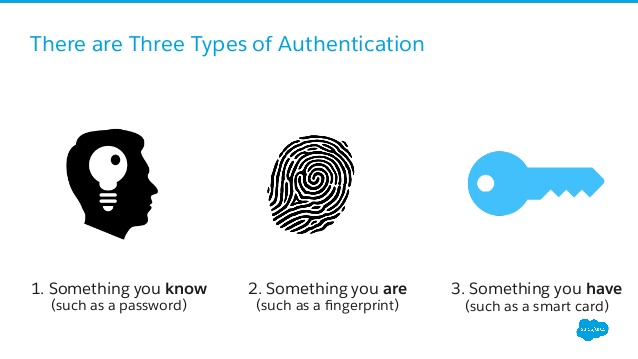
\includegraphics[height=4cm]{3ways.jpg}
\caption{Metode de autentificare \cite{3ways-auth}}
\end{figure}

\subsubsection{JWT}

Majoritatea aplicațiilor de azi se folosesc de cea mai simplă formă de autentificare,
prin folosirea de credentiale (ceva ce utilizatorul știe) și unui token de acces (ceva
ce utilizatorul deține). Utilizatorul își creeza cont pentru o anumită aplicație, folosește
credeințalele pentru a se loga, cererea de autentificare ajunge la server unde se verifică
credențialele iar apoi se generează un token care va fi folosit de utilizator pentru a accesa
diferite resurse în aplicație.

Scenariu descris anterior se referă la folosirea de JWT (JSON Web Token), un standard (RFC 7519) \cite{rfc-7519} 
adoptat de multe aplicații mobile în zilele noastre. 
JSON Web Token este o metodă sigură de autorizare a trasferului
de informații între două părți \cite{jwt}, deobicei 
clientul mobil și serverul la care se face cererea. Clientul revendică de la server
o dovadă, un token, care apoi este folosit de client pentru a accesa diferite 
resurse.

Din punct de vedere tehnic, un JWT are urmatoarea forma 11111.22222.33333 și este
alcătuit din 3 parți:

\begin{enumerate}
    \item Antetul (Header)
    \item Datele utile (Payload)
    \item Semnătura (Signature)
\end{enumerate}


\begin{figure}[H]
    \begin{minipage}[c]{0.5\textwidth}
        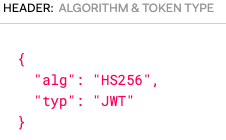
\includegraphics[width=\textwidth]{jwt-header.png}
    \end{minipage}\hfill
    \begin{minipage}[c]{0.5\textwidth}
        \caption{Antetul unui JWT, alcatuit din tipul de algoritm 
        de înregistrare (HS256) și tipul de token (JWT).}
    \end{minipage}
\end{figure}

\begin{figure}[H]
    \begin{minipage}[c]{0.5\textwidth}
        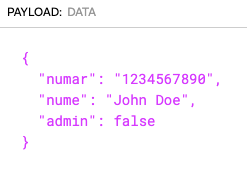
\includegraphics[width=\textwidth]{jwt-payload.png}
    \end{minipage}\hfill
    \begin{minipage}[c]{0.5\textwidth}
        \caption{Partea utilă al unui JWT conține date sau permisiuni
        pe care clientul le are.}
    \end{minipage}
\end{figure}

\begin{figure}[H]
    \begin{minipage}[c]{0.5\textwidth}
        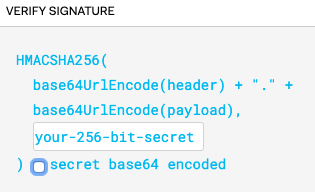
\includegraphics[width=\textwidth]{jwt-sign.png}
    \end{minipage}\hfill
    \begin{minipage}[c]{0.5\textwidth}
        \caption{Semnătura unui JWT este alcătuită din antetul encodat, 
        datele encodate, algoritmul folosit în antet și un secret. Semnătura are rolul
        de a oferi o metodă de verificare pentru a asigura ca conținutul nu a fost 
        modificat }
    \end{minipage}
\end{figure}

\begin{figure}[H]
    \begin{minipage}[c]{0.5\textwidth}
        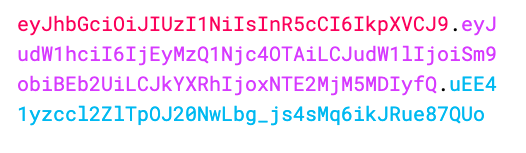
\includegraphics[width=\textwidth]{jwt-all.png}
    \end{minipage}\hfill
    \begin{minipage}[c]{0.5\textwidth}
        \caption{
            JWT va fi format în final 
            de 3 siruri de caractere de tip Base64-URL separate prin punct. }
    \end{minipage}
\end{figure}

O dată ce clientul deține un token, acesta trebuie tratat cu multă grijă 
în cadrul unei aplicații. Acesta poate fi folosit mai apoi în antetul tuturor 
cererilor de tip HTTP sub formă "Authorization: Bearer <token>", din acest motiv 
cel mai probabil se dorește salvarea token-ului în memoria locală a dispozitivului
pentru a putea fi apoi folosit în viitor. Acesta poate fi criptat iar la rândul 
lui la nivelul clientului, deși în mod nativ atât pe android cât și pe ios există metode
sigure de stocare a datelor de tip primitiv (SharedPreferences în mod private pe Android și
keychain pe iOS).

Pentru un nivel și mai mare de siguranță, se poate limita durata de timp
pe care este valabil un token. Spre exemplu aplicația BT Pay folosește un token
care este valid tip de 10-15 minute. După ce token-ul expiră, utilizatorul este nevoit
să se autentifice din nou.

Avantajul principal pe care îl oferă JWT este facilitatea prin care se demarează tot procesul
de revendicare a datelor sau drepturile de la un server de catre client.  
Un alt aspect important îl reprezintă faptul că în spate, totul se produce folosit obiecte
de tipul JSON, fapt ce il face extrem de ușor de implementat și folosit in orice limbaj
de programare.

\subsubsection{Autentificare prin senzori biometrici}

Biometria este termenul tehnic folosit pentru măsurătorile și calculele făcute legate
de corpul uman. Se folosește de metrici legate de caracteristicile umane. În cazul
dezvoltării de software, biometria este folosită pentru autentificare.

Autentificarea prin senzori biometrici se folosește de un factor moștenit, ceva ce îl definește pe
utilizator și prin urmare este una dintre cele mai comode și rapide metode de autentificare.
Mai mult decât atât, datele biometrice precum aprentă sunt greu de furat sau compromis.

Din ce în ce mai multe aplicații încep să folosească autentificare prin senzori 
biometrici, un factor major îl joacă faptul că în ultimi ani, capabilitățile hardware ale
dispozitivelor mobile a crescut exponențial, telefoanele vin încorporate cu diferinti
senzori biometrici precum: senzori de amprenta și recunoaștere facială (iris și rețină).

Metricile biometrice pot varia de la caracteristici fizice pânâ la aspecte ale 
comportamentului unei persoane. În cea ce privește dispozitivele mobile putem idetifica
trei tipuri de autentificari biometrice:

\begin{enumerate}
    \item Senzor de amprentă, extrem de sigur deoarece fiecare individ are
    o amprentă unică.
    \item Recunoașterea vocii, avantajoasă deoarece nu necesitâ hardware in plus dar
    nepotrivit pentru situații unde utilizatorul trebuie să păstreze liniștea.
    \item Recunoaștere facială, la fel ca cea a vocii, nu necesită hardware adițional dar 
    nepotrivit pentru locuri în care luminozitatea este scăzută. 
\end{enumerate}


Utilizarea senzorilor biometrici implică anumite aspecte de care un dezvoltator de
aplicații mobile trebuie să țină cont:

\begin{itemize}
    \item Verificarea ca dispozitivul mobil este încorporat cu senzorii folosiți,
    în cazul în care un dispozitiv nu are senzorii biometrici, dezvoltator trebuie 
    să ofere o metodă alternativă de autentificare. \cite{enisa-2017}
    \item Cererea de permisiunea petru folosirea senzorilor.
    \item Verificarea datele biometrice asociate dispozitivului să nu se modifică
    de la prima autentificare. Această măsură trebuie luată pentru a împiedică cazuri
    în care se adaugă noi date biometrice (amprenta nouă).
\end{itemize}

Deși autentificare prin senzori biometrici este mai rapidă și comodă, această nu ar trebuii
să înlocuiască în mod complet autentificare făcută la nivel de server. 
Ambele metode pot coexista în funcție de context.

\begin{figure}[H]
\centering
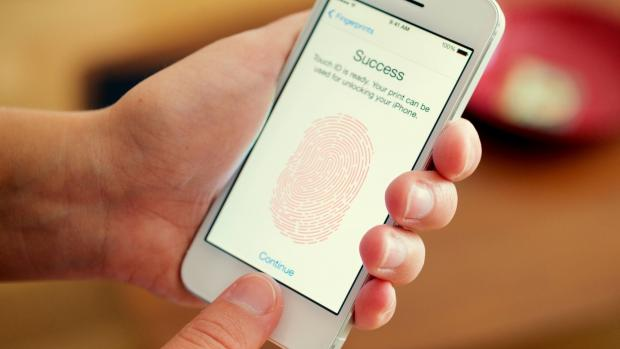
\includegraphics[height=4cm]{fingerprint-smartphone_0.jpg}
\caption{Autentificare prin senzor de amprentă}
\end{figure}


\newpage
\subsubsection{Autentificare prin factori multiplii}

Autentificare prin factori multiplii (MFA) este un sistem de securizare a autentificării
prin impunerea a mai multor metode de verificare a identității unui utilizator.

Autentificare prin factori multiplii combină mai multe metode independente de autentificare.
Așa cum am văzut în capitolul anterior, autentificarea prin senzori biometrici și autentificarea
prin credentiale lucrează cel mai bine împreună. Pe această idee, rolul autentificării prin factori
multiplii este acela de a creea un sistem greu de compromis în vederea asigurării siguranței și
confidentialitații datelor utilizatorului. Astfel dacă unu din componentele sistemului este compromis,
atacatorul este oprit de restul barierelor. În cazul în care cineva are acces la credentialele unui 
utilizator și la dispozitivul sau mobil, atacatorul poate fi oprit prin folosirea senzorului de amprenta.

Un alt caz de utilizare al autentificarii prin factori multiplii îl reprezintă autentificarea în doi pași
sau OTP (one time password). Rolul autentificarii în doi pași este acela de a crea o barieră în plus
în sistemul de securizare al autentificarii prin creeare de coduri/parole temporare unice.

După ce un utilizator se loghează folosind credențialele valide, un cod unic și temporar este generat
și trimis utilizatorului prin diferite canale, deobicei prin SMS, email sau aplicații special făcute
pentru generarea de coduri unice. Utilizatorul este apoi nevoit să introducă codul primit pentru
a își confirmă identitatea. Utilizarea sa nu se limitează doar la autentificare, ci poate fi folosită în
mod general pentru a confirmă identitatea persoanei. Un exemplu îl reprezintă aplicațiile financiare care
atunci când se încearcă o plata, vor trimite un cod unic pentru a verifică identitatea persoanei care 
a inițiat acțiunea.

Deși folosirea autentificarii prin doi pași este destul de comună în cadrul aplicațiilor mobile, această metodă
prezintă și anumite vulnerabilități, mai ales când canalul de comunicare a parolei este prin SMS sau prin 
apel telefonic.
SMS-urile pot fi interceptate și redirecționate, la fel și apelurile telefonice. În astfel de cazuri
se poate limita valabilitatea codului primit la un iterval scurt de timp (5-10 minute). 

Utilizarea unui sistem de autentificare multiplu precum autentificare în doi pași este de altfel recomandată
și de ENISA \cite{enisa-security-data-processing} într-un studiu făcut în vederea 
siguranței procesării datelor personale de către companii mari.

\begin{figure}[H]
\centering
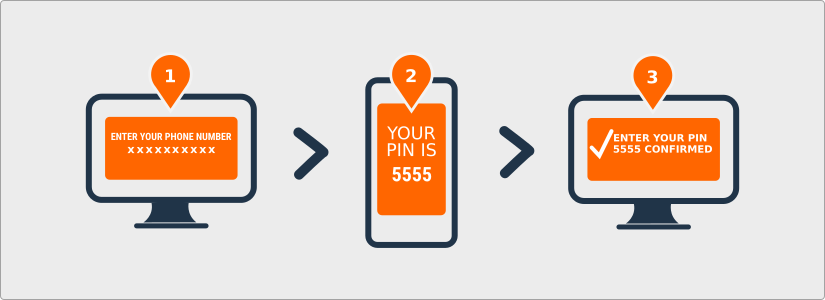
\includegraphics[height=4cm]{wordpress-two-factor-authentication.png}
\caption{Autentificare în doi pași}
\end{figure}

\subsection{Permisiuni}

Permisiunile sunt un aspect important în vederea păstrării condifentialitatii datelor utilizatorului.
O aplicație poate cere o anumită permisiune în diferite cazuri, pentru a accesa date personale (contacte, mesaje)
sau pentru a accesa anumite funcționalități și senzori (apeluri telefonice, camera, senzori biometrici).

În medie un dispozitivil mobil are instalate 95 de aplicații, fiecare aplicație având nevoie
de 5 permisiuni \cite{liu2016follow}. Problematica permisiunilor este adesea ignorată și de utilizator
și de dezvoltatorul aplicației. 
În trecut, pe dispozitivele cu sistem de operare Android, când o aplicație trebuia
să determine SSID-ul rețelei curente nici o permisiune nu era necesară. Acest lucru putând duce la
determinarea locației utilizatorului bazat pe numele și SSID-ul rețelei \cite{ssidloc}. Spre exemplu dacă rețeau s-ar numi
"Gara Nord București", locația utilizatorului ar fi putut fi dezvăluită fără permisiunea lui. În versiunile noi de Android,
determinarea SSID-ului se poate face doar dacă utilizatorul a dat consensul pentru
folosirea locației sale.

În același timp, dezvoltatorul aplicației nu trebuie să abuzeze de permisiuni. Cererile directe 
către utilizator ar trebuii să se limiteze la funcționalitățile aplicației. Spre exemplu, o aplicație
de timp calculator nu ar avea nevoie de permisiunea pentru apeluri telefonice.

Pentru a combate astfel de cazuri, google a început dezvoltarea unui algoritm pentru 
determinarea dacă o aplicație folosest ein mod eronat anumite permisiuni \cite{googleperm}.

\begin{figure}[H]
    \centering
    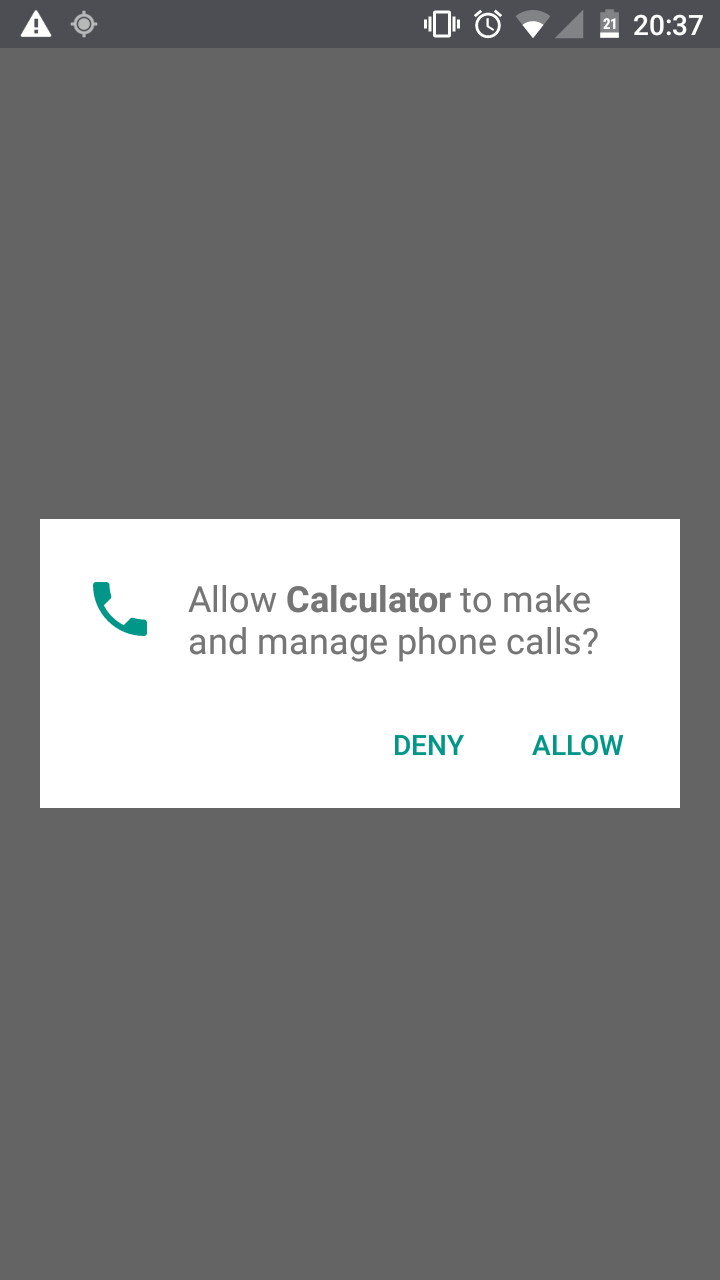
\includegraphics[height=8cm]{calc.png}
    \caption{Abuzarea de permisiuni \cite{redditcalc}}
    \end{figure}

Pentru o gestiune corectă a permisiunilor se mai recomandă următoarele:

\begin{itemize}
    \item Cererea unei anumite permisiuni să aibe loc doar atunci când este strict necesară.
    În cazul în care o aplicație depinde în mod permanent de o anumită permisiune (permisiunea de locație pentru aplicații de navigare),
    atunci cererea se poate face la deschiderea aplicației.
    \item Trebuie luat în considerare și diferitele versiuni ale sistemului de operare. Atât pe Android cât și pe iOS
    pot fi necesare diferite permisiuni pentru aceași acțiune. Exemplu cu SSID amintit anterior.
    \item Folosirea unei singure permisiuni în loc de un întreg grup. De multe ori mai multe permisiuni sunt
    grupate penru a facilita cererea lor. Dar în cazul în care doar un element din grup este folosit atunci este 
    recomandat folosirea doar a elementului respectiv.
    \item Expunerea în mod clar a motivului necesității unei anumite permisiuni către utilizator.
\end{itemize}


\newpage
\subsection{Canale de comunicare}
\subsubsection{HTTP și HTTPS}

Majoritatea aplicațiilor mobile se folosesc de unul sau mai multe servere pentru a își aduce date
sau pentru a prelucra date preluate de la utilizator. Această practică este folosită pentru a evita  stocarea de
date pe dispozitivele utilizatorului având în vedere memoria limitată pe care o dețin. Din acest motiv 
este necesar folosire unor protocoale de comunicare. Cele mai folosite protocoale de comunicare în ecosistemul
mobil sunt HTTP și HTTPS.

Aceste protocoale de comunicare sunt un set de reguli care descriu modalitatea prin care datele sun trimise și 
primite. În mediul mobil, HTTP și HTTPS sunt cele maifolosite protocoale pentru a trimite text imagini și sunete.

HTTPS este varianta sigură a lui HTTP, pe tot parcursul comunicării, datele sunt criptate de la un capăt la altul.
Deși HTTP este mai frecvent folosit, este recomandată folosirea protocolului HTTPS mai ales pentru aplicații 
care gestionează date sensibile.

Dezavantul folosirii protocolului HTTPS îl reprezintă performanță. Criptare și decriptarea datelor trasmise sunt
operații costisitoare. Deși există o pierdere de performanță, există studii \cite{goldberg1998comparison} care demonstrează
că diferența de performanță este modestă, și încurajează folosirea protocolului mai sigur. Un alt studiu \cite{felt2017measuring}
arată că pe anumite sisteme de operare mobile, precum Android, rata de adopție pentru HTTPS este în urmă față de rata de adopție
pe desktop. 

\begin{figure}[H]
\centering
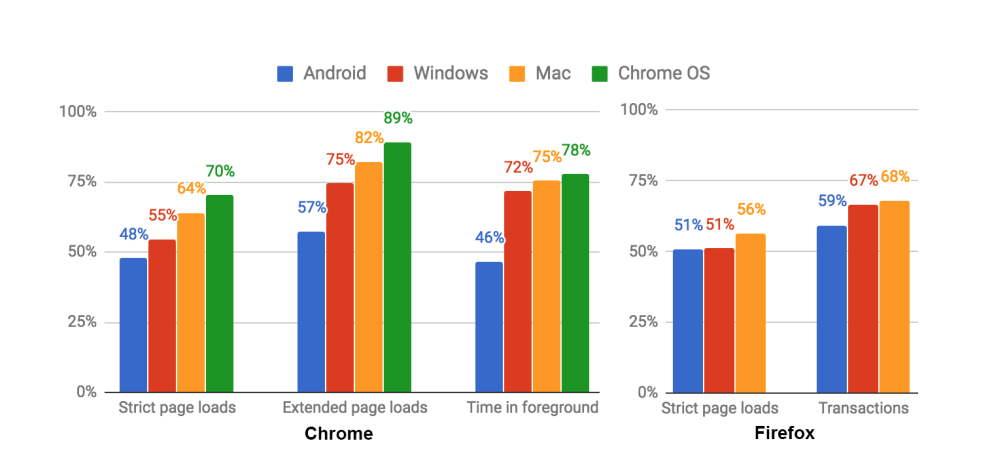
\includegraphics[width=15cm, height=7cm]{http.png}
\caption{Procentul de utilizare HTTPS pe diferite sisteme de operare la sfarsitul unei saptamani din
Febraruie 2017 \cite{felt2017measuring}}
\end{figure}

\subsubsection{SMS}

SMS (Short Message Service) este un serviciu folosit de majoritatea dispozitivelor mobile. Cazurile de 
utilizare ale serviciului variază de la simpla folosire pentru a comunica mesaje scurte, până la 
autentificare cu parolă unică. În 2010, 6.1 trilioane de mesaje au fost trimise cu o medie de 193.000 de SMS-uri
pe secundă \cite{riseof3g}. 


Din punct de vedere tehnic, SMS este un protocol de comunicare care permite schimbul de mesaj scurte. Un SMS 
poate fi format din 160 de caractere alfanumerice, mesajele mai mari de 160 de caractere sunt sparte în 
mai multe mesaje. 
Un mesaj trimits este mai întâi interceptat de SMSC (Short Message Service Center) care de cele mai multe ori
este menținut de providerii de rețele telefonice. SMSC-ul trimite mai apoi mesajul către un alt SMSC (al receptorului)
mesaj pe care în final îl trimite receptorului.

În ciudat popularității sale, comunicare prin SMS prezintă
anumite vulnerabilități. Cel mai periculoasă vulnerabilitate 
este "SMS spoofing". Aceasta are loc când un atacator manipulează
adresa mesajului pentru a impersona pe cineva. Aceste tipuri de
atacuri pot fi prevenite prin verificarea datelor emițătorului 
înainte că mesajul să ajungă la receptor. O altă metodă de protejare,
adoptată mai ales în cadrul autentificării prin 2 pași, este folosirea unui
SMS gateway, servicii special dedicate pentru astefel de operații, dotate
cu diverse măsuri de protecție.

\subsubsection{WebSocket}

Standardizat în 2011 în RFC 6455 \cite{fette2011websocket}, WebSocket este
un protocol de comunicare bidirecțional bazandu-se defapt o conexiune de tip TCP.

Principalul avantaj pe care îl oferă protocolul WebSocket este facilitatea
prin care se permite trasferul de date în mod bidirecțional. În comparație cu protocolul HTTP,
un server poate transmite date unui client fără ca acesta să fie făcut o cerere.

La fel ca HTTP, protocolul WebSocket (WS) este dublat de variată protejată WSS, oferind
criptare de la un capăt la altul al comunicării.

Când vine vorba de aplicații mobile, WebScocket-urile sunt folosite
predominant de aplicații care au nevoie de o comunicare de tip broadcast. 
Aplicațiile de mesagerie în grup precum WhatsApp folosesc WebSocket-uri pentru
a notifica toți utilizatorii unui grup de mesajele noi primite.

Deși WebSocket rezolvă probleme de conectivitate, nu rezolva și problemele de 
securitate \cite{erkkila2012websocket}. vulnerabilități la nivelul acestui protocol
variază de la simple interceptări ale datelor în rețea, atunci când se folosește varianta
neprotejată a protocolului, până la vulnerabilități mai severe precum blocarea serviciului
(DDos) \cite{test-ws}. Pentru a evita astfel de probleme este sugerată folosirea variantei
protajate (wss) și limitarea conexiunilor sau verificarea conexiuniilor când provin din aceasă sursă.


Fiind o tehnologie încă tânăra, WebSocket încă nu este la fel de răspândit
precum HTTP sau SMS, dar că orice sistem de comunicare, includerea lui într-o
soluție soft necesită atenție sporită pentru a prevenii eventuale probleme de securitate.


\newpage
\subsection{Persistența datelor}
\subsubsection{Metode de persistare a datelor}

Una din principalele atribuții a majoritatea aplicațiilor mobile
este aceea de a gestiona și/sau stoca datele utilizatorului. Fie că 
vorbim de aplicații cu servicii web dedicate sau jocuri simple, toate aplicațiile
au nevoie de o metodă pentru persistare datelor. 

Deși modalitatea de persistare a datelor diferă în funcție de platforma
(iOS sau Adroid), se pot extrage câteva caracteristici generale comune.

Dezvoltatorul aplicației trebuie să decidă unde și cum va stoca datele,
în funcție de gradul lor de confidențialitate și tipul de dată. Folosirea
în mod eronat a sistemelor oferite de platforma pe care se dezvoltă aplicația
poate duce la expunerea de date sensibile.

Există mai multe metode prin care se pot salva datele și unde pot apărea
vulnerabilități din punct de vedere al securității:

\begin{enumerate}
    \item Fișiere Log, scopul lor, în mod normal, este acela de a păstra
    un jurnal al activității pentru o anumită aplicație, fiind ușor
    accesibile. Date sensibile pot fi expuse în mod involuntar prin astfel de fișiere (credentiale, token-uri, 
    date primite din cereri HTML).
    \item Baze de date locale SQL. Folosite pentru a păstra
    un volum mai mare de date. Pe ambele platforme există variate necriptate și criptate.
    \item Fișiere folosite pentru setări (SharedPreferences și NSUserDefaults). Folosite
    pentru a stoca date de dimensiune mică cum ar fi valori pentru setări. La fel că 
    bazele de dată SQL, există variante criptate și necriptate. Trebuie menționat
    că atunci când fișierele de preferințe sunt folosite pentru a stoca date de autentificare (token-uri) 
    este recomandată folosirea variantei criptate.
    \item Memoria internă, sistemul de fișiere intern al dispositivului poate fi folosit
    pentru a păstra date. Deobicei se poate folosii pentru a păstra fișiere publice de tip 
    multimedia, cum ar fi poze sau videoclipuri.
    \item Memoria externă (doar pe Android), asemănătoare cu memoria internă, 
    disponibilă prin folosirea de carturi SD sau alte extensii hardware.
\end{enumerate}

Majoritatea metodelor enunțate anterior sunt protejate într-un fel sau altul
de sistemul de operare. În cazul dispozitivelor mobile modificate (jailbreak sau rooted), 
sistemele de protecție oferite de sistemul de operare ajung a fi compromise.

\subsubsection{Criptografie}

Dupa cum am vazut pana acum, multe aspecte ale unei aplicatii mobile pot fi securizate
prin folosirea de elemente native securizate, librarii sau implemtarii proprii. Toate acestea
au la baza o caracteristica comuna, criptarea datelor.

\bigskip

După cum am văzut până acum, multe aspecte ale unei aplicații mobile pot fi securizate
prin folosirea de elemente native securizate, librării sau implemtarii proprii. Toate acestea
au la baza o caracteristică comună, criptarea datelor.

\bigskip

Criptografia este studiul tehnicilor matematice legate de aspectele 
securității informațiilor, cum ar fi confidențialitatea, integritatea datelor, 
autentificarea entității și autentificarea originii datelor \cite{katz1996handbook}.

Problematica securității informației nu este una modernă, de a lungul istoriei 
au fost nevoie de diferite metode de securizare a informației, mai ales în timp de război.
Deobicei implica păstrarea datelor într-o maniere incopresibila. Pentru a decripta
astfel de mesaje, se puteau folosii diferite tehnici de decodare.

Criptografia modernă se rezumă la algoritmi bazați pe teorie matematică, greu 
de spart datorită complixitatii și ipotezelor pe care se bazează. Practic astfel de
algoritmi pot fi sparți dar necesită o putere de calcul foarte mare.

Deși există multe tehnici folosite în criptarea datelor, cea mai populară și folosită
în zilele noastre este criptarea prin cheie publică (criptografie asimetrică), folosită
de instituii guvernamentale, armata și corporații mari.


Criptografia asimetrică presupune folosirea a două chei, una pentru criptarea datelor
(cheia publică) și una pentru decriptarea datelor (cheia privată). Fiecare receptor are o cheie privată unică pe care o folosește pentru a de cripta datele.
Emițătorul oferă cheia publică oricui, folosită pentru a cripta datele. Cheia publică și privată sunt deobicei într-o relație matematică dar calcularea lor
nu este fezabilă.

\begin{figure}[H]
    \centering
    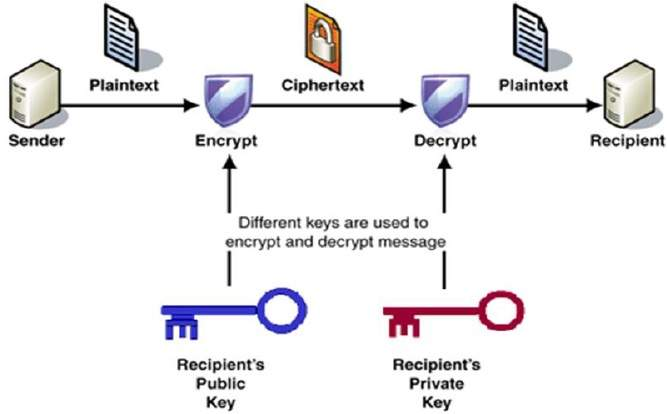
\includegraphics[height=6cm]{public_key_cryptography.jpg}
    \caption{Criptografie Asimetrică \cite{tutrsa}}
    \end{figure}

RSA (Rivest–Shamir–Adleman) este cel mai folosit cripto sistem cu cheie publică. Relația matematică 
dintre cele două chei este securizată prin alegerea a două numere prime foate mari care sunt păstrate secrete \cite{barton2012regulation}.


\newpage
\section{Medicarium}
\subsection{Analiza aplicației}
\subsubsection{Problematica}


"Mobile Health" (m-health) \cite{kahn2010mobile}
este termenul folosit pentru a descrie utilizarea tehnologiilor mobile precum telefoanele pentru
a sprijinii și îmbunătății sistemul de sănătate. Aplicațiile mobile au un potențial foarte mare când vine vorba de medicină, cazurile lor
de utilizare variază de la simpla monitorizare a unor aspecte medicale până la 
comunicare între doctori, pacienți și instituții medicale.

În ultimii ani dispozitivele mobile au început să fie dotate cu din ce în ce mai mulți
senzori pentru a oferii mai mult suport pentru astfel de aplicații. Creșterea în popularitate a adus ca urmare anumite reglementări.
În iulie 2011, Administrația Statelor Unite pentru Alimente și Medicamente a emis un proiect de orientare privind 
reglementarea aplicațiilor medicale mobile \cite{barton2012regulation}. Astfel se propune ca aplicațiile
mobile medicale trebuie să gasesasca un echilibru intre înbunatațirea calității vieții utilizatoriilor și 
respectarea siguranței și confidențialității.


Medicarium este o aplicație care își propune centralizarea istoricului medical al utilizatorilor săi.
În România există deja un astfel de sistem pin "Cardul de Sănătate". Din păcate nu toate persoanele din România 
au primit astfel de carduri, mai mult de cât atât, viitorul acestui sistem nu este cert. O altă problema a cardului
de sănătate este faptul că utilitatea lui este limitată la sistemul de sănătate public
din România.

Luând aceste probleme în calcul, Medicarium poate fi folosit oriunde, de oricine indiferent
că vorbim de sistemul public sau private și indiferent de țară.

În prima faza Medicarium va fi folosit pentru a păstra istoricul medical al pacientului. 
Sunt stocate date generale ale pacientului (grupa de sânge, greutate, vârstă etc\dots), 
cat si documente medicale (analize, teste).

\newpage
\subsubsection{Cazuri de utilizare}

Aplicatia Medicarium permite urmatoarele funcționalități:

\begin{enumerate}
    \item Înregistrare și verificare cont.
    \item Autentificare prin factori multipli (date de logare, pin și senzori biomerici).
    \item Stocarea și editarea datelor medicale generale ale pacientului.
    \item Stocarea documentelor medicale. Utilizatorul poate adaugă noi documente 
    folosind camera sau din galaria telefonului.
    \item Modificarea vizibilității datelor în caz de urgență.
    \item Mod de urgență care paote fi folosit de orice persoană pentru a vedea
    datele medicale pe care utilizatorul le-a setat în prealabil. 
\end{enumerate}


\begin{figure}[H]
\centering
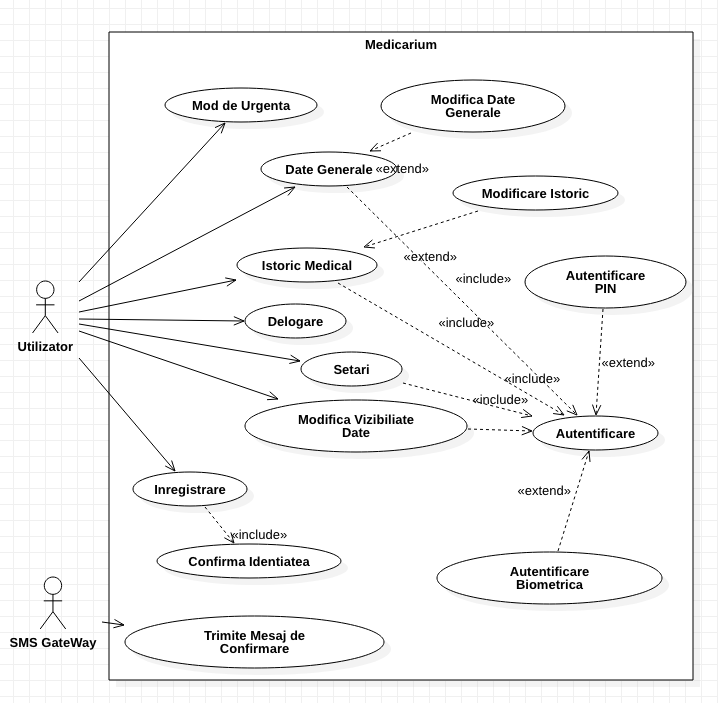
\includegraphics[height=9cm]{cazuri.png}
\caption{Diagrama Cazurilor de Utilizare}
\end{figure}

\newpage
\subsection{Proiectarea aplicației}
\subsubsection{Arhitectura}

Solutia o sa fie compusa din 2 aplicatii mobile, clientul mobil propriu-zis
si un "SMS Slave", o aplicatie separata folosita special pentru a trimite mesaje
pentru autentificarea si verificarea utilizatorilor.

Clientul mobil este accesibil oricui pe cand aplicatia pentru mesaje este privata,
fiind intretinuta impreuna cu serverele si baza de date.

La fel ca aplicatiile, avem doua server, un REST API care satisface cererile primite
de clientii mobili si un SMS Gateway, care intermediaza comunicarea intre serverul REST
si SMS Slave-ul.

Comunicarea intre servere se face prin HTTPS.
Comunicarea intre SMS Gateway si SMS Slave se face prin WebSocket pentru a mentine
un canal de comunicare bidirectional.

Server-ul REST comunica direct cu o baza de date  nonrelationala de tip mongoDB.

\begin{figure}[H]
    \centering
    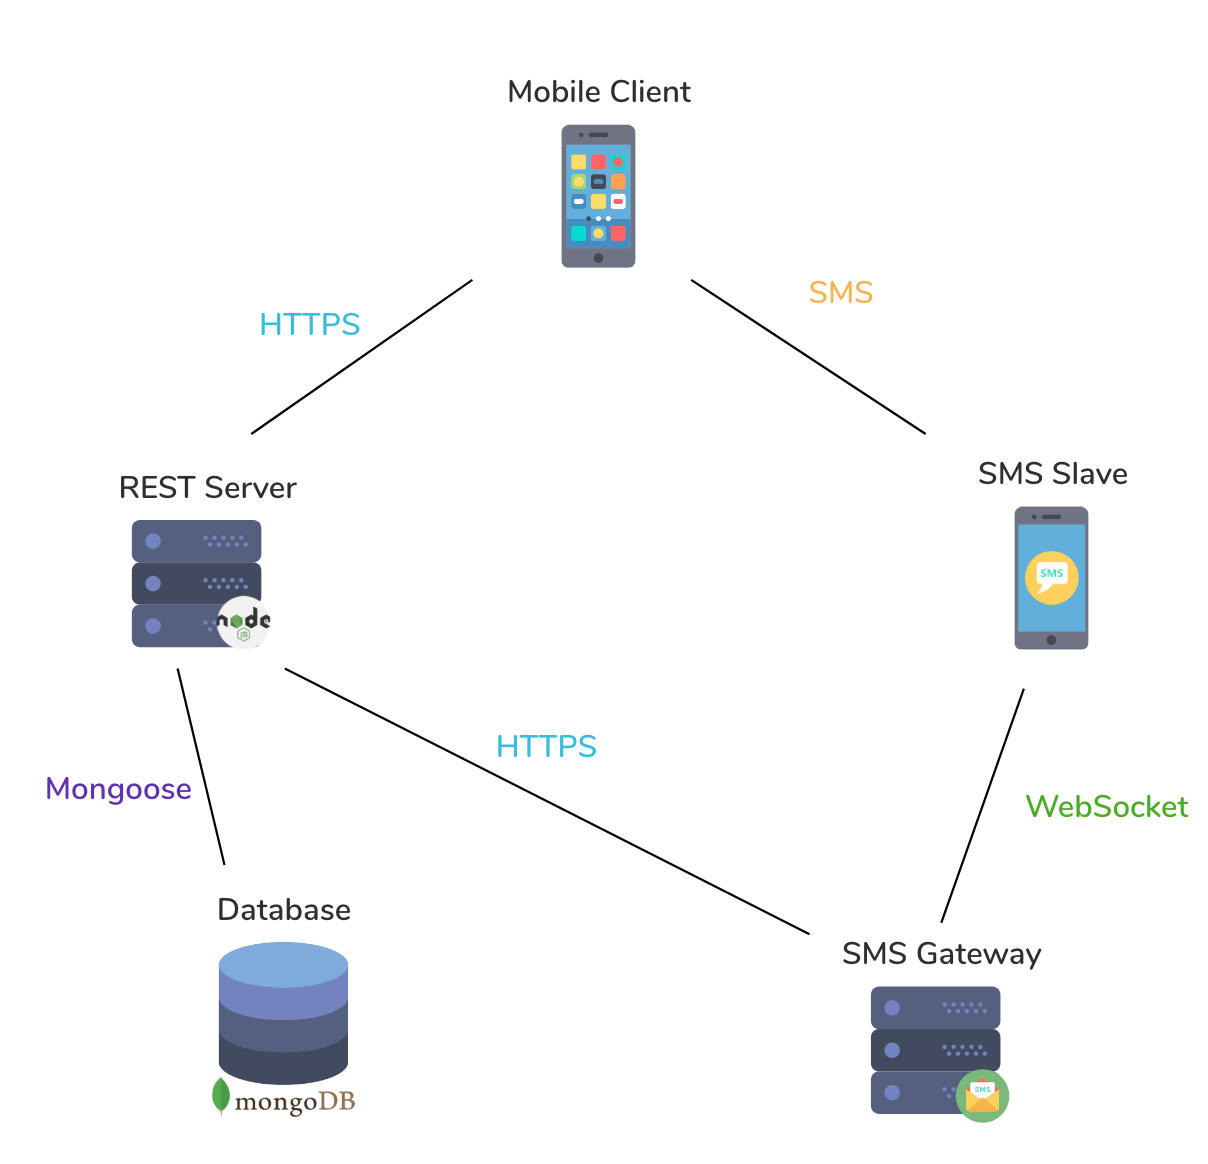
\includegraphics[width=10cm, height=8cm]{arhi.png}
    \caption{Diagrama de arhitectura a aplicatiei}
    \end{figure}

\newpage
Server-ul REST o sa fie impărțit in mai multe module dupa cum urmeaza:

\begin{itemize}
    \item Un modul pentru Modele (Models), cara să conțină difinițiile schemelor 
    entităților din baza de date.
    \item Un modul pentru Rute (Routes), care gestioneaza cererile primite la server
    \item Un modul pentru interceptorul de token (Middleware), cărui rol e sa
    verifice daca cererile către server au un token valid.
    \item Un modul de teste
    \item Modulul principal care cuprinde restul modulelor si contine fișierele server.js
    si index.js a caror scop e să centralizeze restul modulelor
\end{itemize}

\begin{figure}[H]
    \centering
    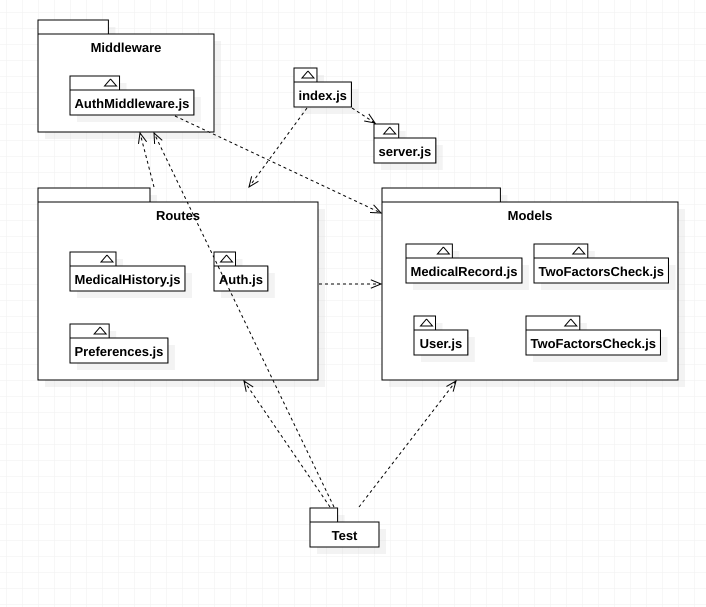
\includegraphics[width=12cm, height=10cm]{pacheteserver.png}
    \caption{Diagrama de pachete pentru server}
    \end{figure}

\newpage
Clientul mobil o să fie și el împărțit in pachete:



\begin{figure}[H]
    \centering
    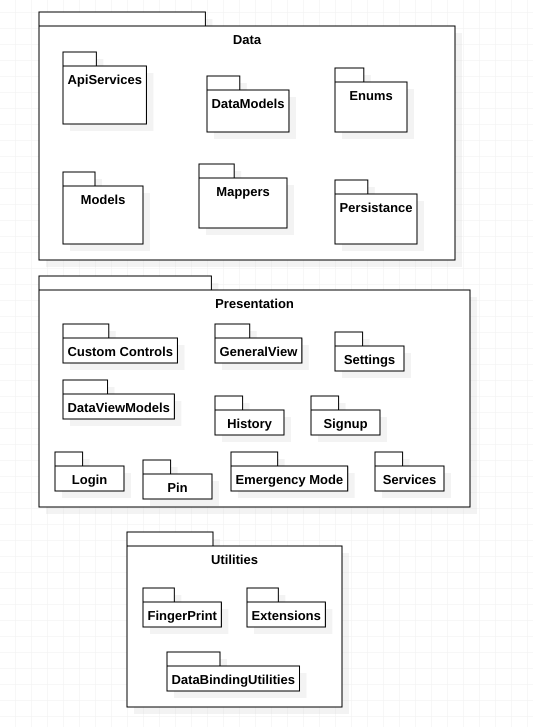
\includegraphics[width=14cm, height=17cm]{pacheteclient.png}
    \caption{Diagrama de pachete a clientului mobil}
    \end{figure}


Conținutul parțial al pachetului Data prin urmatoarea diagramă de clase:


\begin{figure}[H]
    \centering
    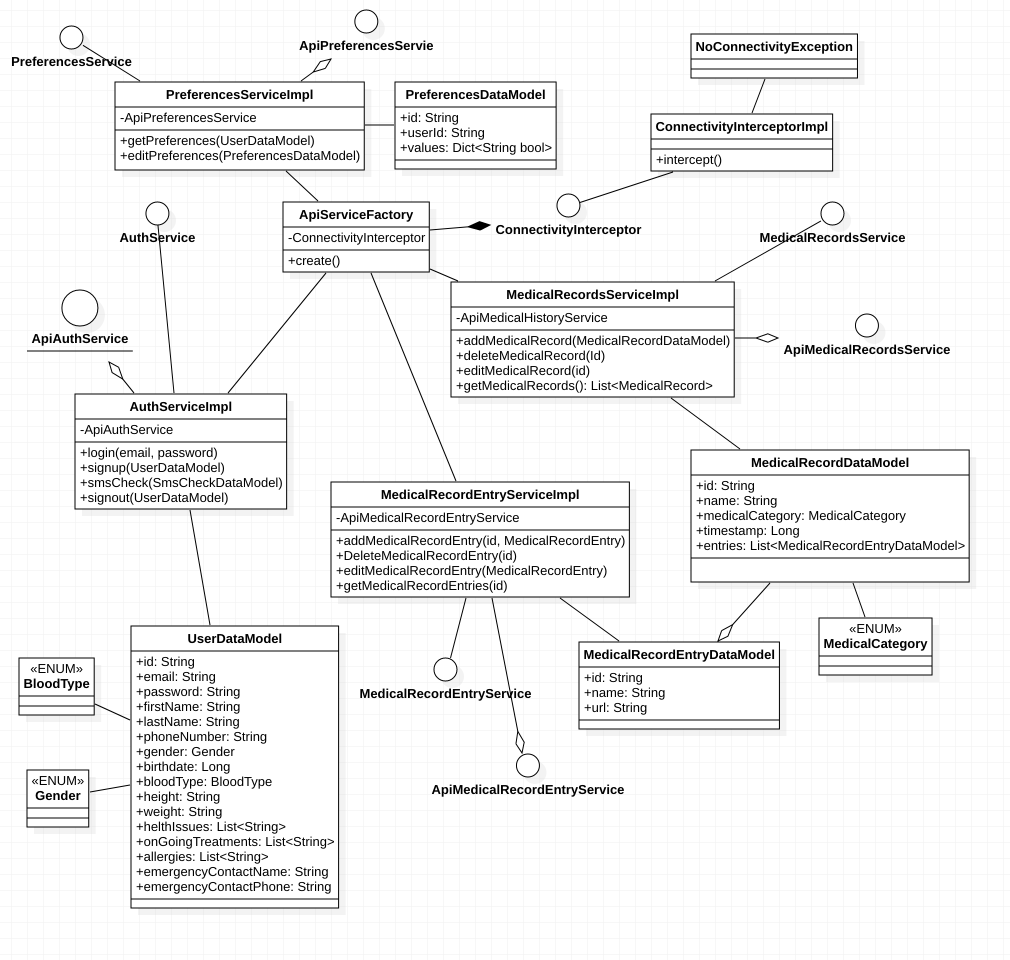
\includegraphics[width=15cm,height=17cm]{dataclase.png}
    \caption{Diagrama de clase parțială a pachetului Data}
    \end{figure}

\subsubsection{MVVM}

Pentru a crea o arhitectură ușor de menținut și ușor de modificat am optat să folosesc
șablonul arhitectural MVVM.

MVVM este un șablon arhitectural original dezvoltat de Microsoft pentru Windows Presentation Foundation (WPF) framework-ul
din .NET destinat dezvoltării de aplicații desktop. Este o variată a MVP-ului, un alt șablon arhitectural.
Este predominant folosit pentru dezvoltarea de aplicații cu interfață grafică. Structural el este alcătuit din 3 componente:

\begin{figure}[H]
\centering
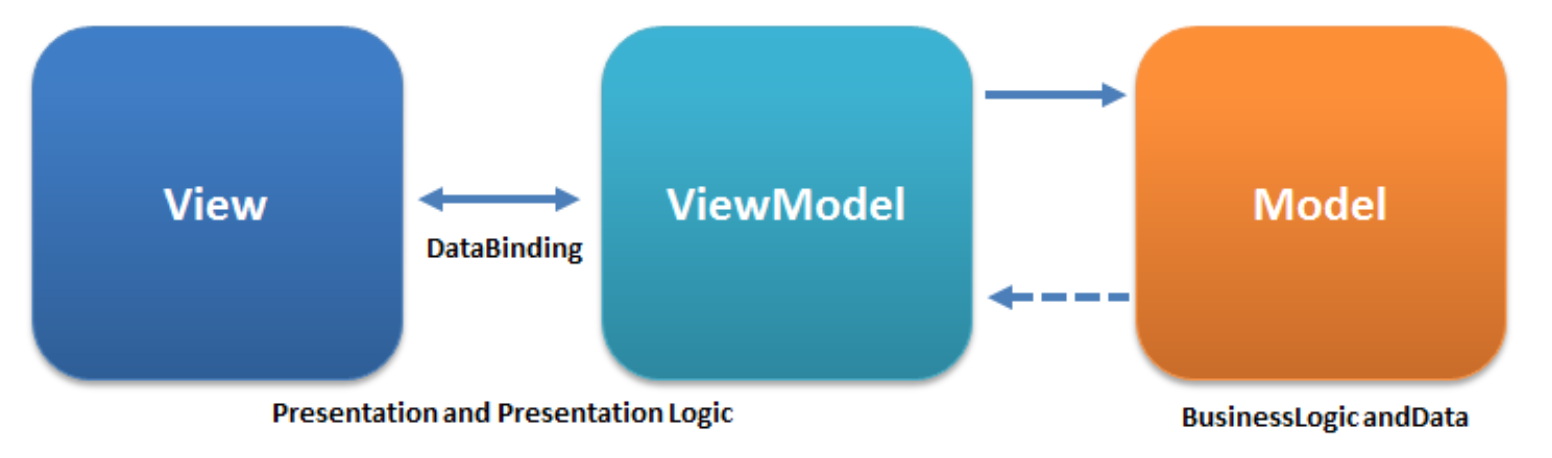
\includegraphics[width=12cm]{mvvm.png}
\caption{Componentele din MVVM \nocite{mvvmpng}}
\end{figure}

\begin{enumerate}
    \item View. Se referă la un ecran sau la o parte din interfață grafică,
    ce e văzut de utilizator. Este responsabil de input-ul dat de utilizator. În cazul aplicației
    Medicarium, view-urile sunt toate ecranele pe care aplicația le are

    \begin{figure}[H]
    \centering
    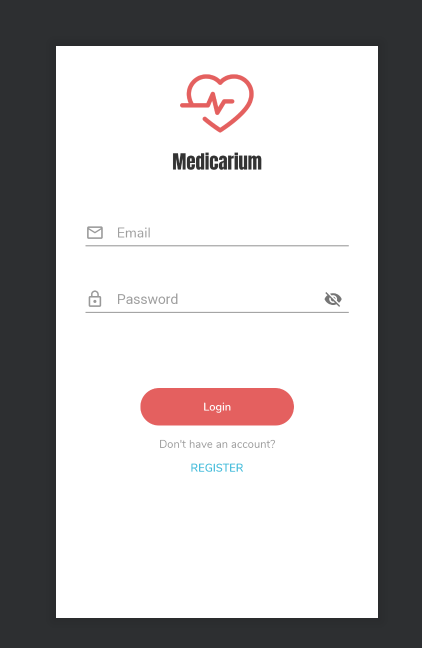
\includegraphics[width=4cm, height=6cm]{view.png}
    \caption{Exemplu de View bazat pe cod XML}
    \end{figure}

    \item ViewModel. Descrie starea datelor din model, care apoi este observată de
    View. Deobicei include un Binder carenotifică View-ul când au loc schimbări în Model.
    ViewModel-ul este decuplat de View, nu are nici o referință la el.

    \begin{figure}[H]
    \centering
    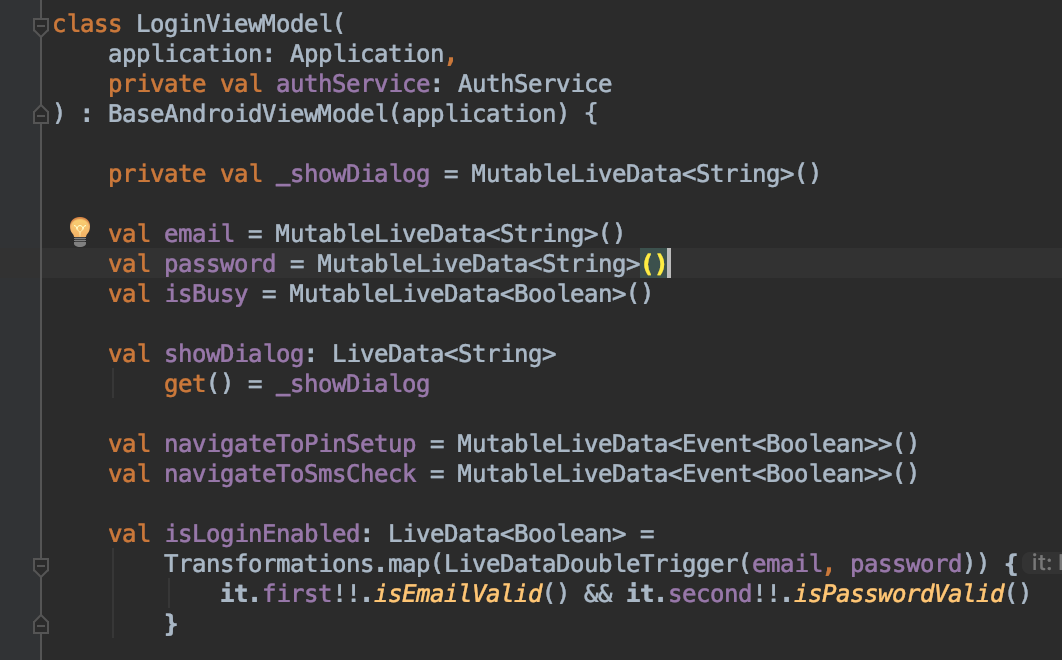
\includegraphics[height=6cm]{viewModel.png}
    \caption{Exemplu de ViewModel pentru View-ul anterior}
    \end{figure}
    
    \item Model. Se referă la datele care sunt observate. Poate
    fi un model din aplicație sau un set de date. Unicul său scop
    e să păstreze datele.


    \begin{figure}[H]
        \centering
        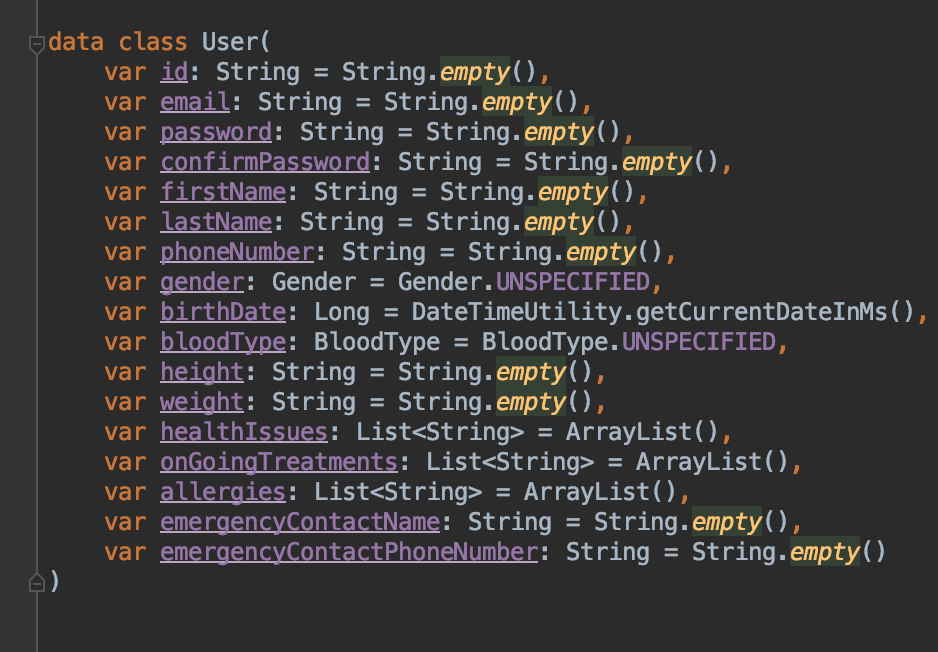
\includegraphics[height=6cm]{model.png}
        \caption{Exemplu de Model din aplicația Medicarium}
        \end{figure}

\end{enumerate}

Deși Google nu impune un anumit stil arhitectural pentru aplicațiile mobile Android, MVP
era cel mai folosit șablon. Asta s-a schimbat recent cu introducerea lui Android
Jetpack, un set de librării care vin să ajute dezvoltatorii de aplicații și care
favorizează folosirea MVVM.

Principalele avantaje a MVVM-ului față de MVP sunt:
\begin{itemize}
    \item O separare mai bună a responsabilităților care implicit duce la o cuplare
    redusă. ViewModel-ul nu are nici o referință la View, el doar oferă o reprezentare
    a datelor care poate fi observată de cineva sau nu.
    \item Ușurează testarea. Componentele fiind redus cuplate între ele pot fi 
    mai ușor testate. ViewModel-ul este o simplă clasa POJO sau POCO care conține
    doar propietăți și metode ușor de testat.
    \item Codul din ViewModel este ușor de refolosit, fâcand MVVM destul de popular pentru proiecte pe diferite platforme.
    \item Cod mai ușor de menținut și mai adecvat pentru metodologii de lucru precum
    agile.
    \item Funcționează foarte bine cu alte șabloane de proiectare (Command, Singleton, 
    Factory etc\dots)

\end{itemize}


\begin{figure}[H]
    \centering
    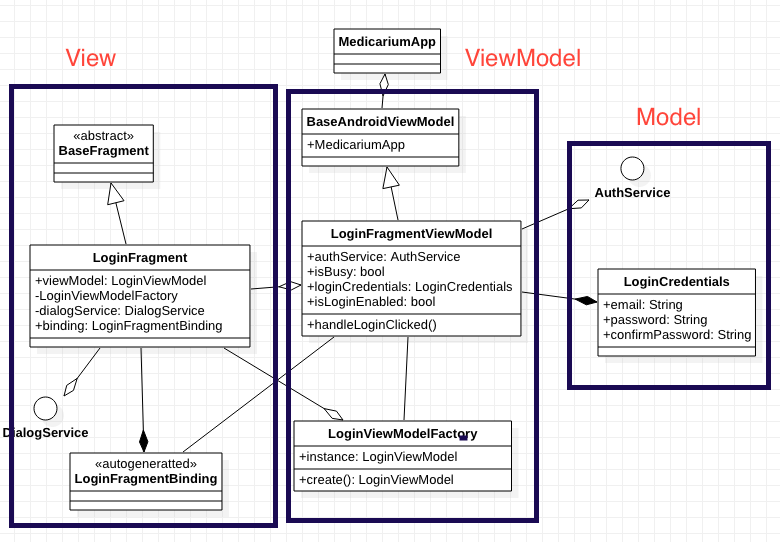
\includegraphics[width=15cm,height=10cm]{mvvmclase.png}
    \caption{Diagrama de clase care evidentiază structura MVVM pentru funcționalitatea de login}
    \end{figure}

Ca orice alt șablon arhitectural și MVVM prezintă puncte slabe:
\begin{itemize}
    \item Mai mult cod. Deși codul devin mai ușor de menținut, cantitatea lui
    poate crește considerabil.
    \item Depanarea codului poate fi anevoiasă datorită sistemului de Databinding.
    \item Poate fi mai greu de înțeles la prima vedere, comparat cu MVC și MVP.
\end{itemize}

Deși MVVM se pretează cel mai bine pentru aplicații mari cu interfață grafică unde testarea este
esențială, poate fi folosit și pentru aplicații de dimensiuni medii. Folosit cum trebuie
poate ajută la o dezvoltare mai rapidă și la o calitate crescută a codului.

\subsection{Implementarea aplicației - Serverul și serviciile}

\subsubsection{Server REST}

Representational State Transfer (REST) este stil arhitectural software care definește
un set de constrângeri pentru creearea de servicii Web. Un serviciu Web este un server web
constriuit pentru a satisface toate nevoile unui site sau unei aplicații \cite{masse2011rest}.

Principala caracteristică a acestor tipuri de servicii îl reprezintă faptul care serverul
nu stochează nici o stare a sesiunii clientului. Fiecare cerere conține toate informațiile
necesare pentru a putea înțelege cererea. Cererile au loc în izolare și sunt idependente, serverul
nu se folosește de informații din alte cereri iar clientul este responsabil pentru trimitarea de
orice dată e necesară pentru a obține răspunsul dorit.

Pricipalele avnataje ale unui serviciu REST sunt:

\begin{itemize}
    \item Suport pentru diferite format de date (JSON, XML, text etc\dots)
    \item Performanță crescută și eficientă, serviciile REST folosesc puțină lățime de bandă
    \item Ușor de modificat, datorită unicității arhitecturii, coponentele sunt izolate
    ușuarând eventuale modificări
    \item Scalabilitate, fiind principalul motiv care a adus la adoptatea serviciilor REST \cite{masse2011rest}
\end{itemize}

În Medicarium, serverul REST este responsabil de a servii clienții mobili cu resurse de
care au nevoie. Există o serie de rute la dispoziția clienților accesibile doar pe baza 
de Json Web Token (JWT). 

\bigskip

Exemple de rute folosite în aplicatiie:

\begin{figure}[H]
\centering
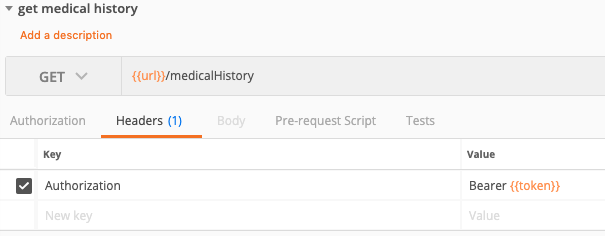
\includegraphics[width=10cm, height=4cm]{get.png}
\caption{Exemplu de metoda GET cu JWT în antetul cererii}
\end{figure}


\begin{figure}[H]
\centering
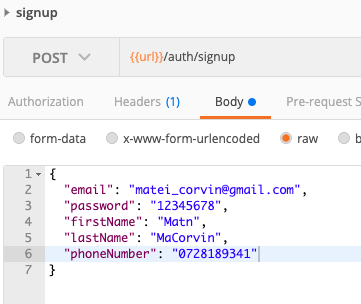
\includegraphics[width=8cm, height=6cm]{post.png}
\caption{Exemplu de metoda POST cu JSON în corpul cererii}
\end{figure}
    
\begin{figure}[H]
\centering

\includegraphics[width=8cm, height=4cm]{delete.png}
\caption{Exemplu de metoda DELETE cu mesaj de eroare}
\end{figure}
    
\subsubsection{Node.js}

Pentru implementarea serverlui REST s-a folosit
Node.js, un mediu de rulare care permite execuția de cod
javascript în afară browser-ului.

Node.js este dublat de npm, un sistem de gestionarea a pachetelor
care permite customizarea unui proiect Node.js cu diferite pachete.

Există numeroase avantaje atunci când se folosește Node.js pentru dezvoltarea unui server.
Fiind javascript, serverul în sine este mai lejer și mai ușor de întreținut. Mai mult
de cât atât, este și mult mai rapid, operațiile de I/O fiind foarte rapide.
Un alt avantaj important îl reprezintă numeroase librării și pachete disponibile în npm.

Servicii mari precum Ebay, Netflix și PayPal \cite{tilkov2010node}, folosesc Node.js, iar popularitatea
acestui stă doar să crească.

\begin{figure}[H]
\centering
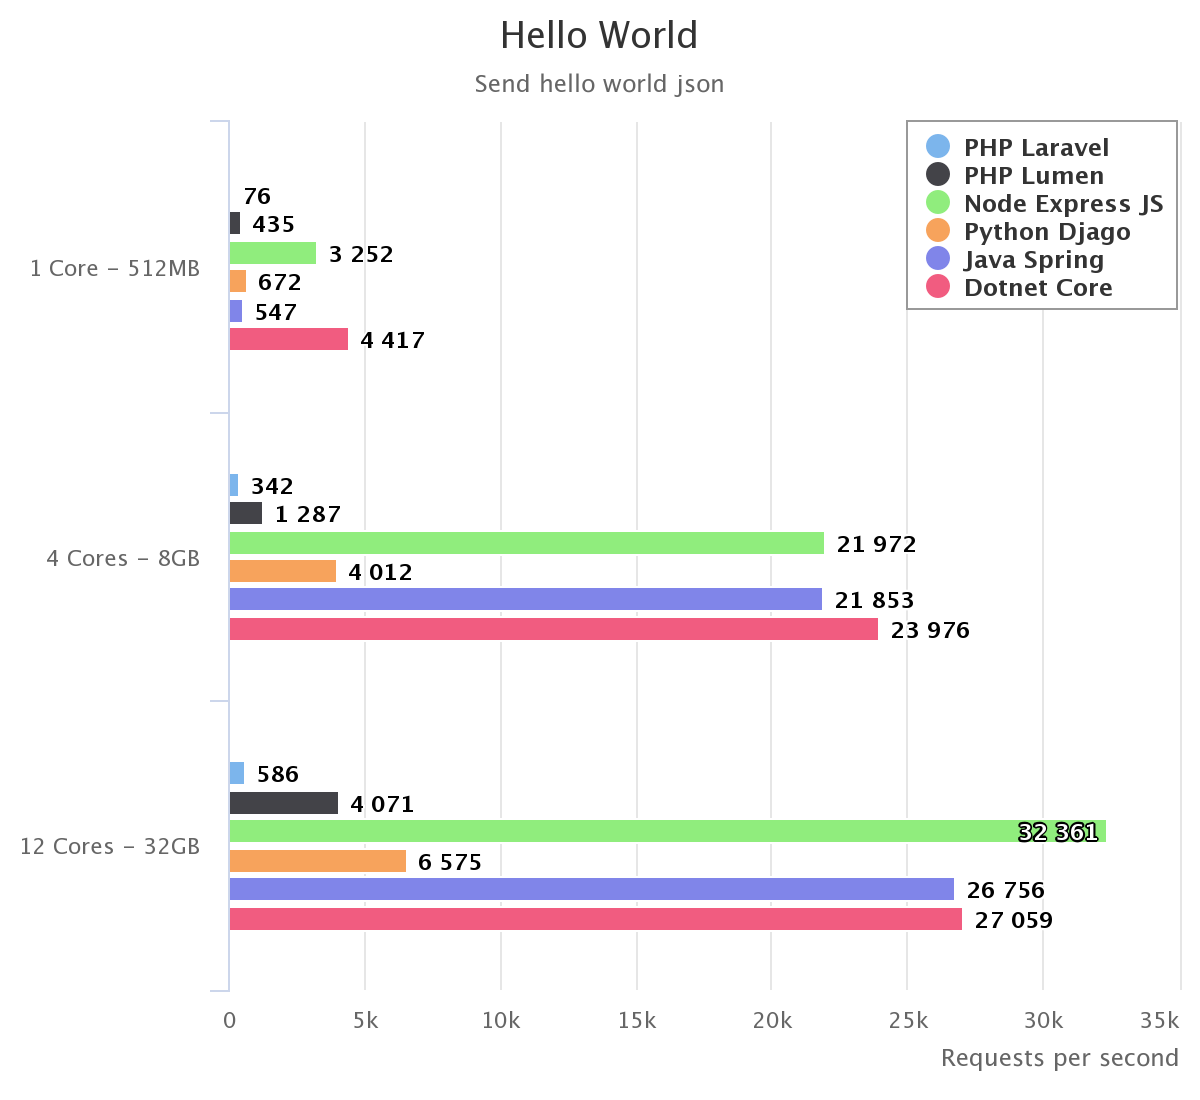
\includegraphics[height=10cm]{nodespeed.png}
\caption{Performanță a diferitor framework-uri \cite{reqpersec}}
\end{figure}

\newpage
\subsubsection{MongoDB}

MongoDB este un tip de baza de date flexibi și scalabil. Combină abilitatea
de a scala cu o multe funcții secundare precum: indexi secundari, interogări range,
sortări, agregări și indexi geospațiali \cite{banker2011mongodb}.

Mai mult decât atât, MongoDB intră în categoria bazelor de date non 
relaționale (NoSSQL). Astfel de baze de date oferă alternative când vine vorba
de modelarea datelor, nu înlocuiesc complet sistemul relațional ci doar îl extind.

Câteva din avantaje folosirii unei baze de date NoSQL \cite{nayak2013type}:
\begin{itemize}
    \item Mai rapide și eficiente
    \item Oferă o gama largă de modele de date
    \item Ușor de scalat
    \item Nu necesită administratori de baze de date
    \item Foarte populare și evoluează rapid
\end{itemize}

Există însă și câteva dezavantaje față de o baza de date relațională:
\begin{itemize}
    \item Devenind populare destul de recent, încă sunt imature
    \item Nu există un limbaj standard pentru interogări
    \item Unele interpretări nu respectă ACID
    \item Mentenanță poate fi dificilă
\end{itemize}


Din punct de vedere tehnic, MongoDB lucrează cu "documente", obiecte de tip JSON care 
mapează entitatiile din aplicație. Este important de precizat că nu există o stuctură
pe care documentele care mapează aceași entitate trebuie să o respecte. Spre exemplu, putem aveam
două documente diferite care mapează o persoana, unul să conțînă doar numele și vârstă, iar al doilea să conțînă
nume, vârstă și înălțime. Acest lucru permite o scalabilitate mai ușoară și în general este mai
ușor de lucrat direct cu obiecte de tip JSON.

\bigskip

În aplicația Medicarium, folosirea unei baze de date MongoDB facilitează în primul rând comunicare
între toate entitățiile care se ocupă de datele aplicației.
Un alt avantaj pe care îl aduce aplicației este eficientă și rapiditatea cu care sunt aduse datele.
Diferența de tip pe care o aduce la citirea si scrierea de date conteaza foarte mult pentru o aplicație mobilă.

Acest sistem implica toate partile solutiei soft, de la aplicatia in sine, pana la
aplicatia dedicata sa trimita doar mesaje.

\begin{figure}[H]
\centering
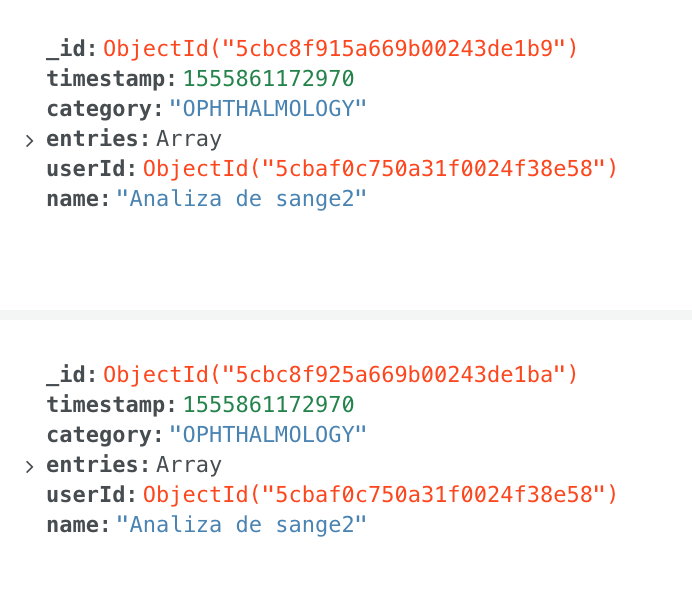
\includegraphics[height=7cm]{exmongo.png}
\caption{Exemplu de documente păstrate în baza de date}
\end{figure}

\newpage

\subsubsection{Verificarea in doi pași}

Pentru a crește nivelul de securitate al aplicației există un sistem de verificare
în doi pași. Așa cum am precizant în prima parte a lucrării, adăugarea unui astfel de sistem
poate fi foarte benefic pentru aplicații.
Mai mult de cât atât, așa cum este precizat și în studiul făcut de ENISA \cite{enisa-2019}, un
astfel de sistem este recomandat pentru a face aplicația să respecte prevederile aduse în GDPR. 

\bigskip

Un flow detaliat al unei astfel de verificări:

\begin{enumerate}
    \item Un utilizator nou dorește să se înregistreze SAU un utilizator cu cont deja creat
    nu are contul verificat
    \item Serverul REST primește cererea de la clientul mobil și va aduce date din baza de date pentru
    a verifică dacă utilizator are cont verificat
    \item În cazul în care utilizatorul are cont verificat, poate intră în aplicație. În caz contrar,
    o cerere este trimisă la serverul care se ocupă de mesaje (SMS Gateway)
    \item SMS Gateway o să salveze cererea în baza de date și va notifica dispozitivul mobil 
    care se ocupă cu trimiterea de mesaje, care la rândul lui va trimite codul la utilizator.
    \item Utilizatorul primește mesajul și introduce codul în dispozitiv, care apoi v-a fi verificat 
    pe server. Dacă codul este valid, utilizatorul își poate continuă activitatea, altfel o să fie nevoit
    să mai încerce o dată.
    \item Verificarea mai poate eșua dacă utilizatorul nu își verifică codul în decursul a 5 minute, valabilitatea
    codului fiind limitată din motive de securitate
\end{enumerate}

\begin{figure}[H]
\centering
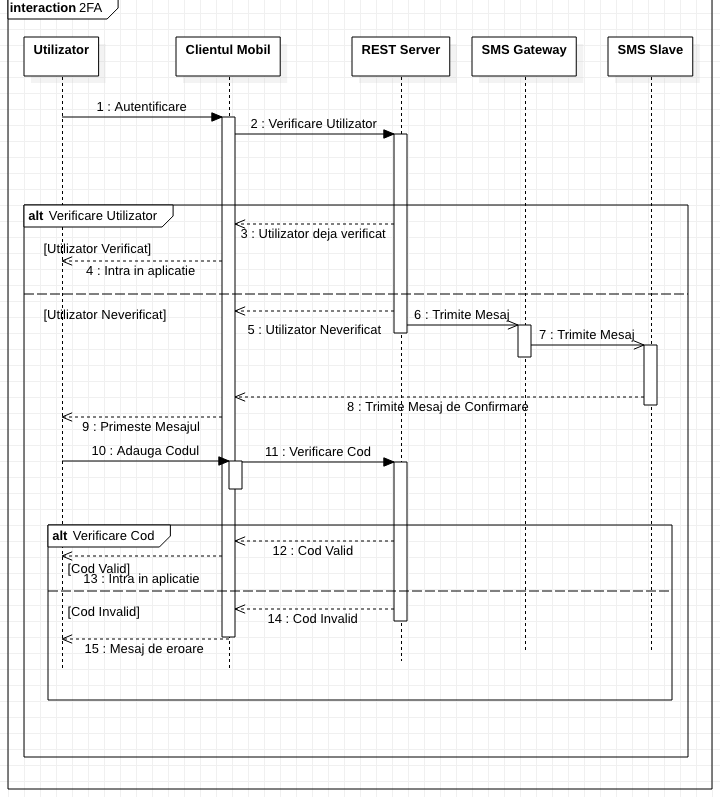
\includegraphics[width=15cm, height=18cm]{2fa.png}
\caption{Diagrama de secvență pentru verificarea în doi pași} (baza de date este exclusă pentru a simplifica diagrama)
\end{figure}


\newpage
\subsection{Implementarea aplicației - Clientul mobil}
\subsubsection{Android Jetpack}

Pentru implementarea ambelor aplicatii, clientul mobil Medicarium si aplicatia pentru mesaje, am optat 
sa dezvolt pe Android, sistem de operare mentinut de Google. Este bazat pe un kernel Linux si este optimizat
pentru a lucra pe device-uri cu touchscreen. 

Mai mult de cat atat, am folosit Android Jetpack,
o colectie de librarii dezvoltate recent care au in vedere imbunatatirea procesului de dezvoltare
a aplicatiilor mobile. 

\begin{figure}[H]
\centering
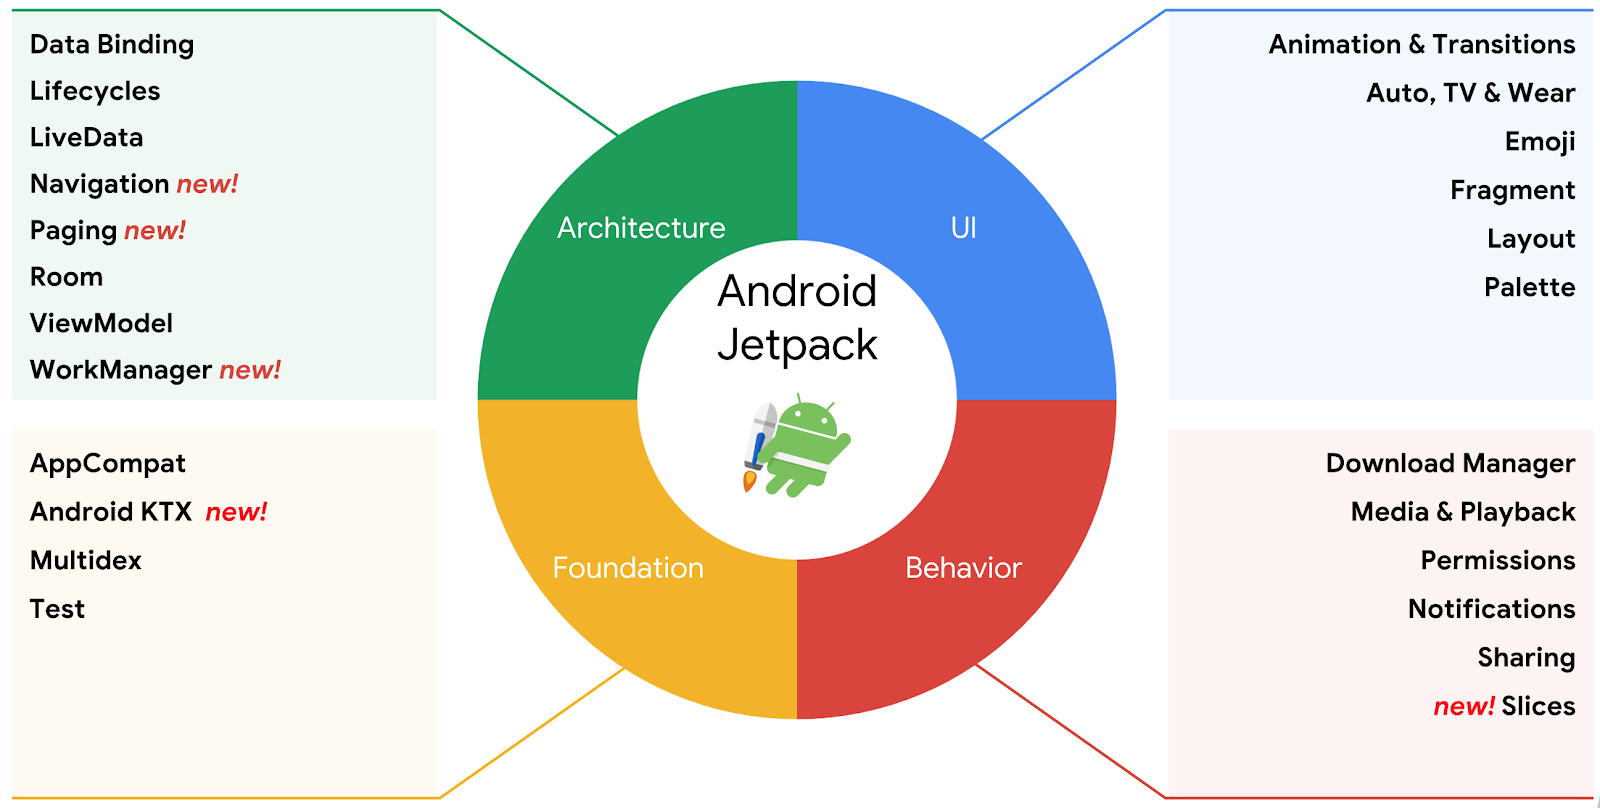
\includegraphics[width=12cm, height=8cm]{androidjetpack.png}
\caption{Componentele din Android Jetpack \cite{jetpackpng}}
\end{figure}

\bigskip
Motivele folosirii platformei Android:
\begin{enumerate}
    \item Popularitea crescuta a sisemului de operare Android. Conform unei 
    statistici \cite{statcounter} sistemul de operare Android ocupa 75\% din 
    piata mobila, pe cand iOS doar 22\%
    \item Sistemul de operare Android este mai vulnerabil de cat iOS. Acest
    lucru se datoreaza faptului ca fiecare vanzator de telefoane cu Android
    are tendinta de a modifica putin sistemul de operare pentru al ajusta nevoilor
    proprii. Sistemul in sine este mentinut doar de Google, astfel se creaza discrepante
    intre diposizivele mobile cu acelasi sistem de operare dar producatori diferiti
    de hardware. Pe de alta parte, Apple detine controlul si al software-ului (sistemul de operare iOS) 
    si al hardware-ului, fiind mai usor de impus masuri de securitate intr-un sistem inchis.
\end{enumerate}

\subsubsection{Kotlin}

Daca pana acum nu mult timp sigura metoda pentru a dezvolta aplicatii pentru Android era Java, in ultimii
ani un nou limbaj este disponibil, Kotlin. Kotlin este un limbaj care a aparut din dorinta de a rezolva
anumite probleme de proiectare pe care Java le are si pentru a imbunatatii procesul de dezvoltare.

Kotlin este un limbaj nou, stabil care poate functiona pe orice device cu Android si rezolva multe
probleme pe care Java nu a putut. Aduce multe concepte in plus, este un limbaj a carui scop e sa faca
viata dezoltatorilor mult mai usoara \cite{moskala2017android}. Kotlin ruleaza pe JVM facand astfel ca orice cod scris in Java sa fie 100\% compatibil.

Cateva avantaje pe care le ofera Kotlin fata de Java:
\begin{itemize}
    \item Cod mai putin. Kotlin este un limbaj mai concis, codul este mai usor de scris
    si citit, crescand astfel eficienta dezvoltatorilor si reducand codebase-ul.
    \item Suport pentru programare functionala. Exista numeroase constructii si concepte
    ale programarii functionale care pot fi folosite in Kotlin.
    \item Null safety. In compartie cu Java, in Kotlin orice obiect care poate avea asignata 
    valoarea null trebuie marcat cu nullable in caz contrar codul o sa esueze la compilare.
    \item Complet compatibil cu Java, trecerea de la Java la Kotlin fiind triviala.
    \item Multe alte concepte moderne (operatori ternari, corutine, extensii de metode etc\dots)
    
\end{itemize}


\begin{figure}[H]
    \centering
    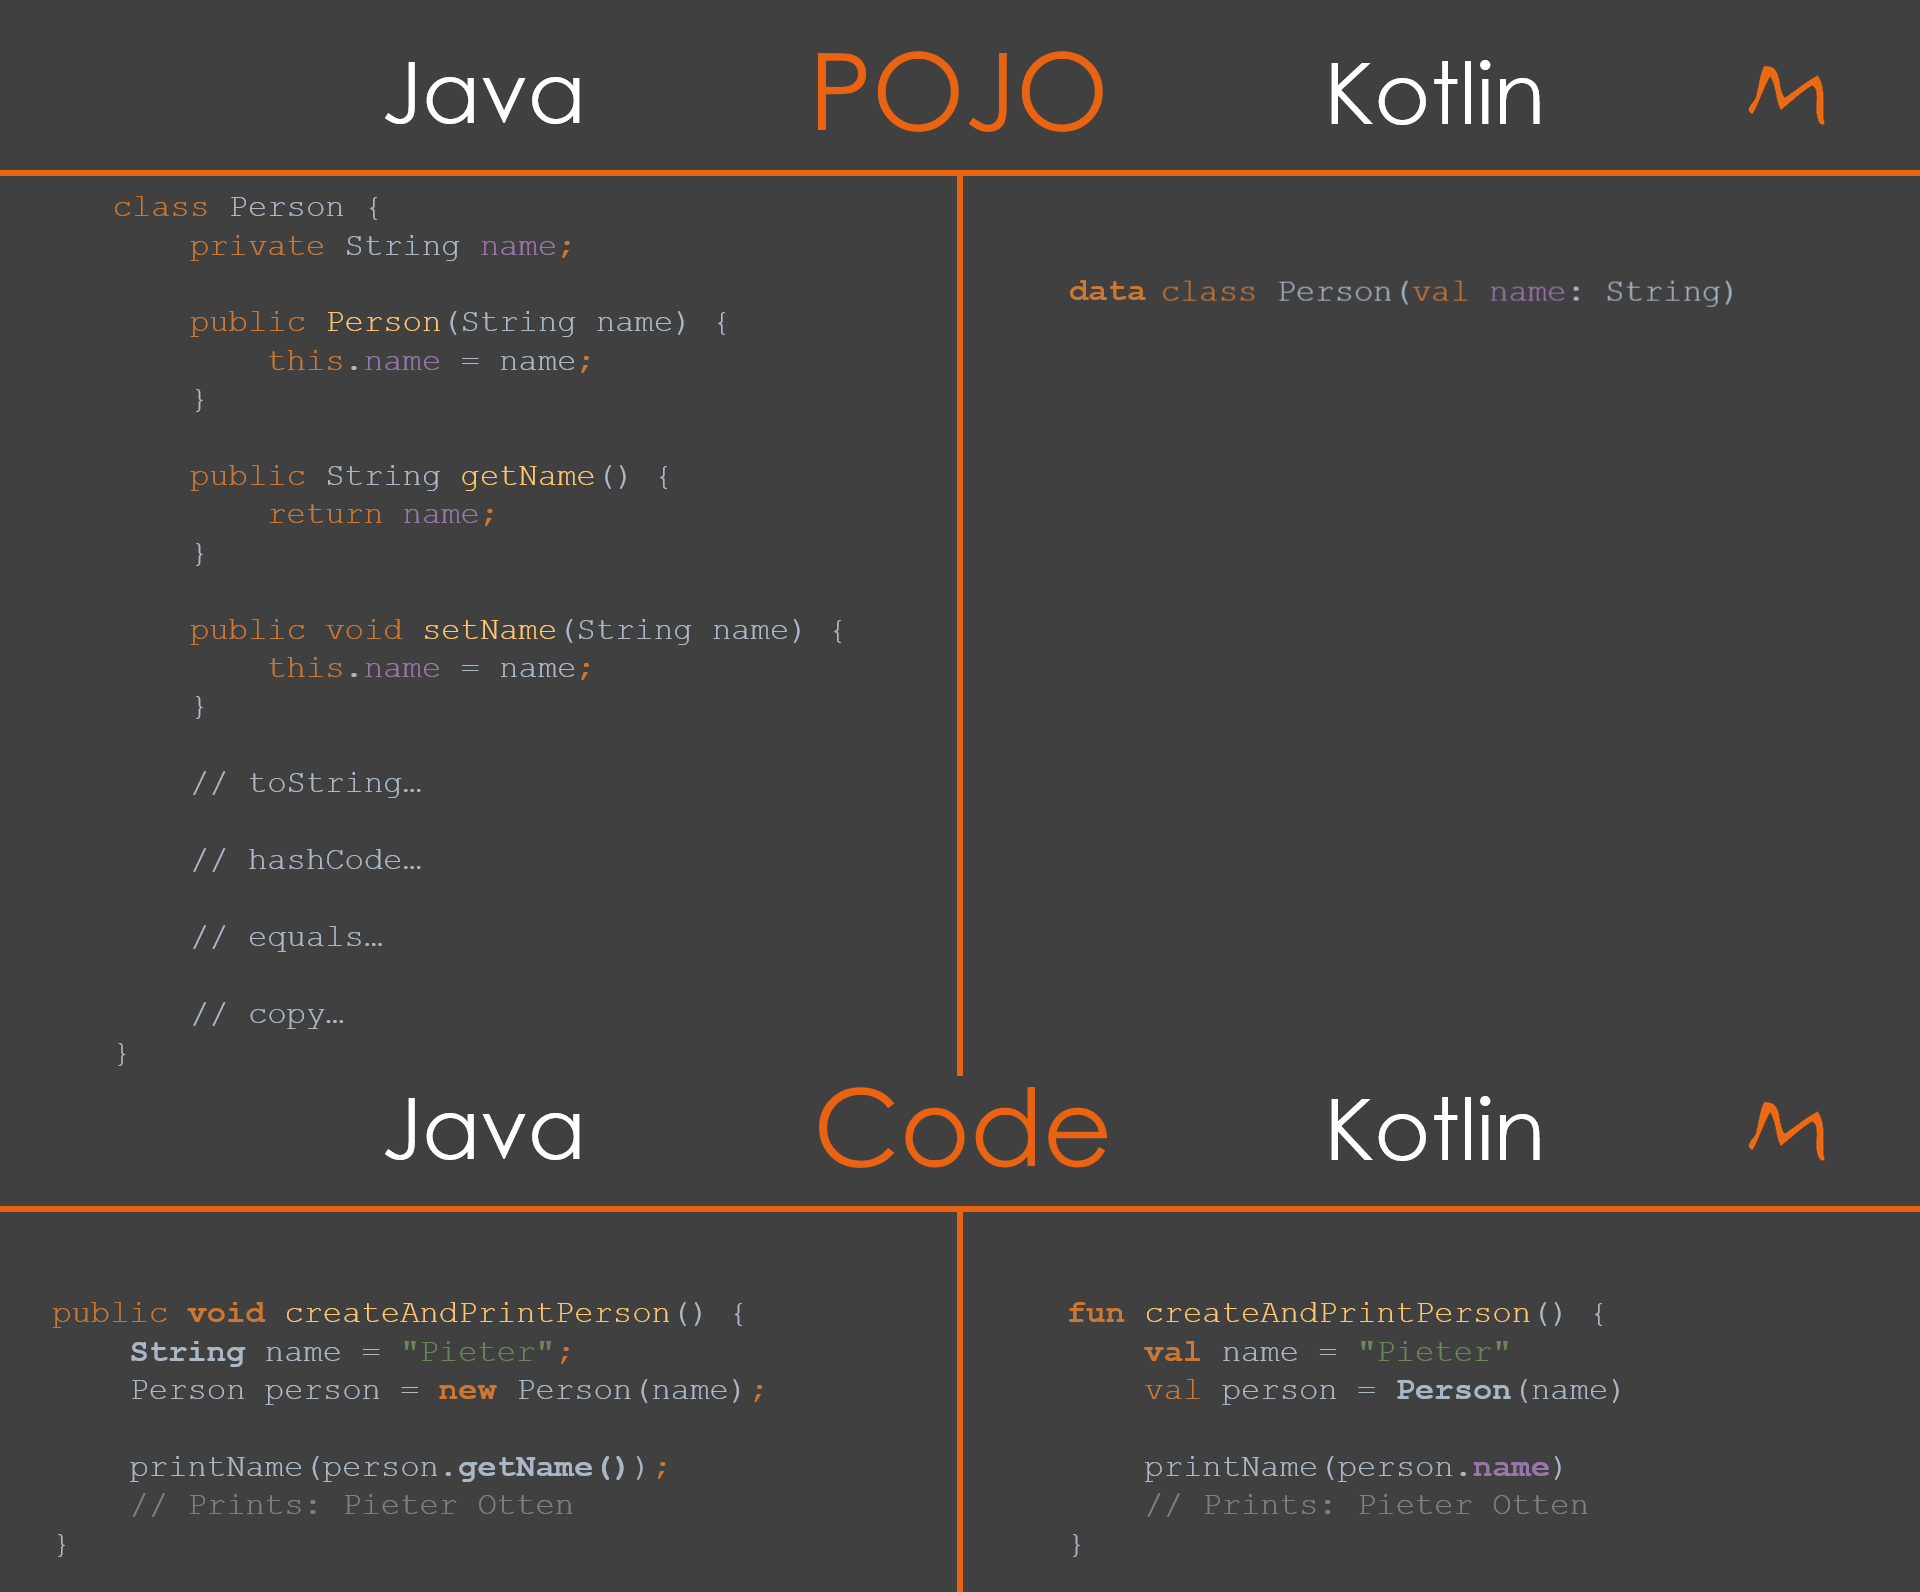
\includegraphics[width=12cm, height=8cm]{kotvsjava.png}
    \caption{Comparatie intre cod Java si cod Kotlin \cite{kotlinvsjava}}
    \end{figure}
    
Multe librarii au inceput deja migrarea din Java in Kotlin. Iar Google a anuntat ca limbajul principal
pentru Android a devenit in mod oficial Kotlin.

\newpage
\subsubsection{Implementarea autentificării}
În această ultimă parte vom vedeam cum am implementat în aplicație anumite necesități
discutate în partea teoretic.
Vom începe cu autentificarea și verificarea identității. Ca în orice aplicație, în prima instanța suntem întâmpinați cu două opțiuni, a ne loga cu un cont deja creat sau a
crea un cont nou:

\begin{figure}[H]
    \centering
    \begin{minipage}[b]{0.4\textwidth}
      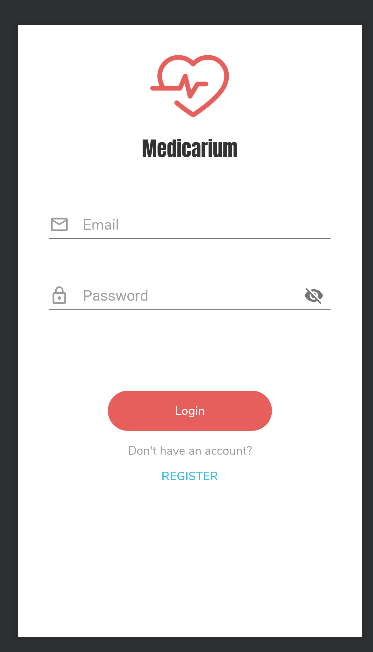
\includegraphics[width=\textwidth]{login.png}
      \caption{Ecranul de Login}
    \end{minipage}
    \hfill
    \begin{minipage}[b]{0.4\textwidth}
      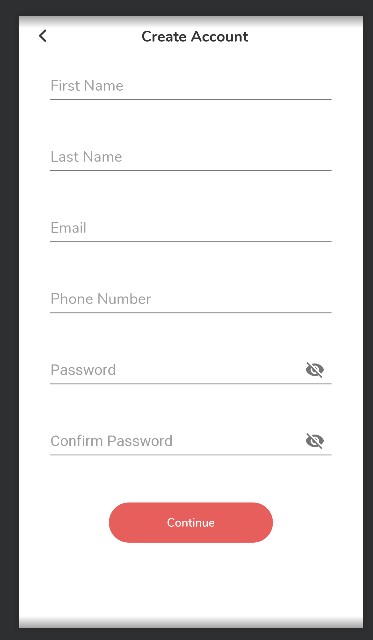
\includegraphics[width=\textwidth]{register.png}
      \caption{Ecranul de Register}
    \end{minipage}
  \end{figure}

În cazul în care contul utilizatorului nu este verificat, un mesaj o să fie trimis
către numărul lui personal pentru a își verifică identitatea. Mesajul este trimis
prin SMS Gateway, serverul separat care se ocupă doar cu trimiterea de mesaje de verificare.

\begin{figure}[H]
\centering
\begin{minipage}[b]{0.4\textwidth}
    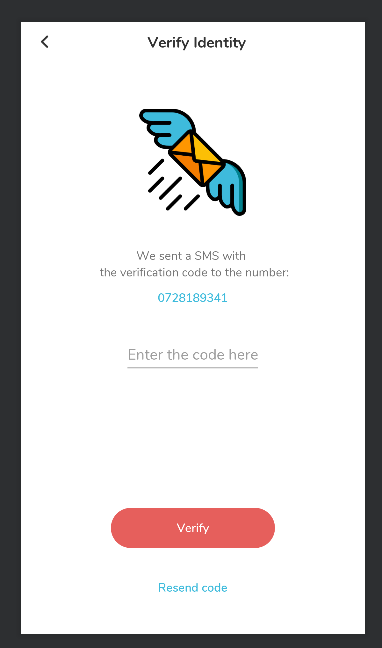
\includegraphics[width=\textwidth]{smsfrag.png}
    \caption{Ecranul de verificare a codului primit prin SMS}
\end{minipage}
\hfill
\begin{minipage}[b]{0.4\textwidth}
    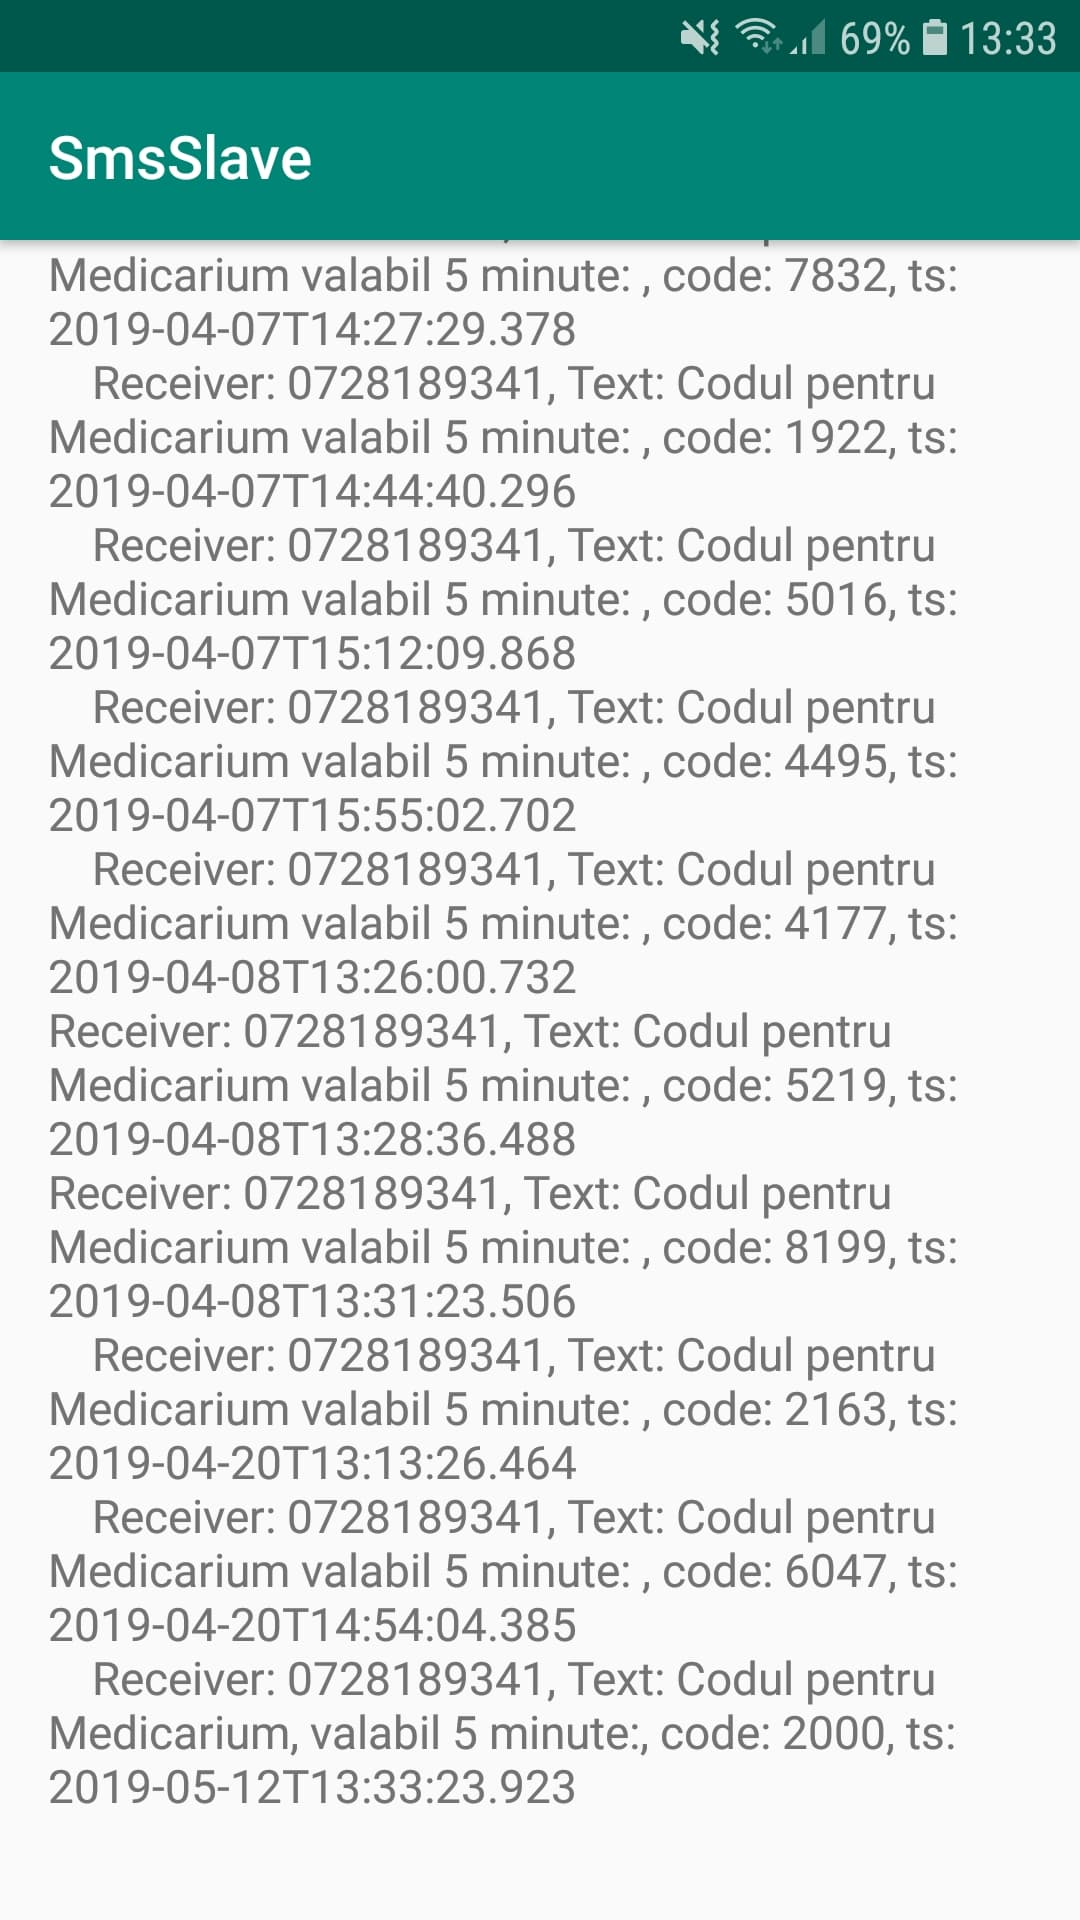
\includegraphics[width=\textwidth]{smsslave.jpg}
    \caption{Aplicația SMS slave}
\end{minipage}
\end{figure}

\begin{figure}[H]
\centering
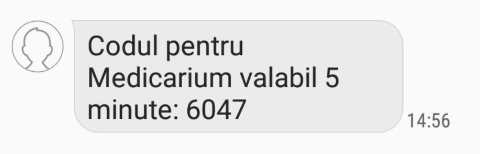
\includegraphics{exsms.png}
\caption{Model de SMS cu cod de verificare}
\end{figure}

O dată ce un utlizator are contul verificat acesta poate intra în aplicație
în dou feluri, prin amprentă sau prin cod PIN. Deși varianta cea mai facilă ar fi prin
aprentă, nu toate telefoanele au senzor astfel în cât se impune necesitatea implementării
și a autentificării prin pin.

\begin{figure}[H]
\centering
\begin{minipage}[b]{0.4\textwidth}
    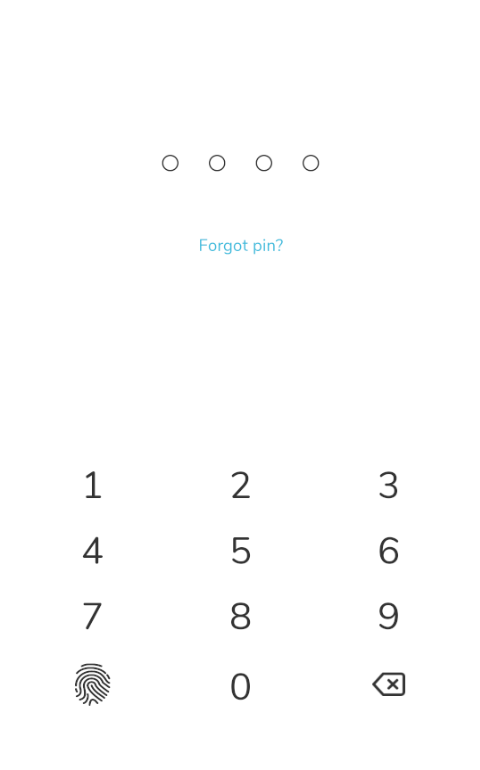
\includegraphics[width=\textwidth]{pin.png}
    \caption{Autentificare prin cod PIN}
\end{minipage}
\hfill
\begin{minipage}[b]{0.4\textwidth}
    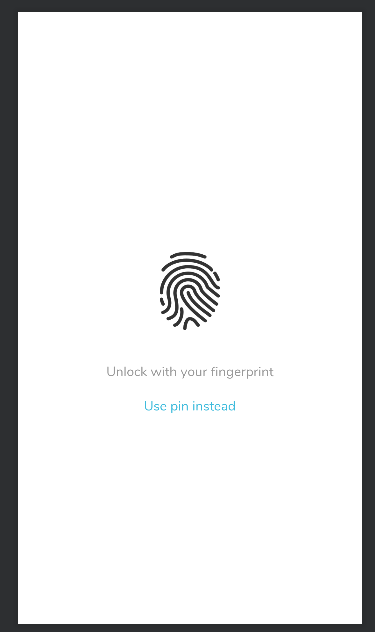
\includegraphics[width=\textwidth]{fingfrag.png}
    \caption{Autentificae prin aprentă}
\end{minipage}
\end{figure}

Pentru a asigura că dispozitivul mobil suportă senzor de amprenta se fac o serie 
de verificări. Se verifică dacă versiunea sistemului de operare este potrivită,
dacă există senzor de amprenta, dacă avem permisiunea de a folosi amprenta utilizatorului
și dacă există cel puțîn o aprentă setată pe dispozitivul respectiv.

\begin{figure}[H]
\centering
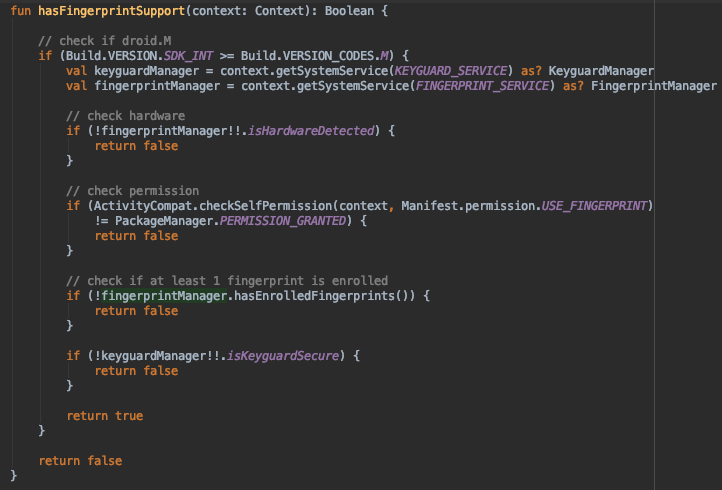
\includegraphics[width=14cm, height=9cm]{fingver.png}
\caption{Metoda care verifică dacă autentificarea prin amprenta este posibilă}
\end{figure}

În cazul în care verificarea prin amprenta nu este posibilă, utilizatorul poate folosi
autentificarea prin cod PIN.

\newpage
\subsubsection{Gestionarea permisiunilor}

Aplicația necestia o serie de permisiuni pentru a funcționa la capabilitățile sale
maxime. Asta nu însemna că fără anumite permisiuni aplicație nu funcționează ci doar o
să limiteze funcționalitățile disponibile. Spre exemplu dacă utilizatorul nu permite
accesul la camera, el o să poată folosii restul aplicație dar nu funcționalitățile care necesită 
camera.

Permisiunile sunt cerute în general atunci când sunt necesare.

\begin{figure}[H]
    \centering
    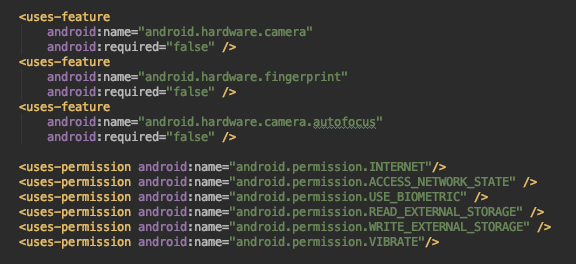
\includegraphics[width=14cm, height=7cm]{listapermi.png}
    \caption{Lista de permisiuni folosite în Medicarium}
    \end{figure}

\begin{itemize}
    \item Permisiunea pentru Internet și starea rețelei sunt folosite
    pentru a accesa rețeau și pentru a verifică dacă există conexiune
    \item Permisiunea la senzorii biometrici și senzorul de amprenta sunt folosite
    pentru autentificare
    \item Camera, autofocusul și accesul la datele externe sunt folosite atunci când se adugă anlize noi
    \item Permisiunea pentru vibrații este folosită pentru a oferii feedback utilizatorului
\end{itemize}

\subsubsection{Persistența datelor și comunicarea cu serverul}

Majoritatea datelor nu sunt păstrate pe dispozitivul utilizatorului ci sunt
trimise direct serverului prin canale siguri de comunicare, folosind HTTPS.

Putem exemplifica un astfel de flow pentru funcționalitatea de "adaugă analiză medicală":

\begin{enumerate}
    \item În prima faza utilizatorul completează datele necesare și sunt validate
    în clientul mobil.

    \begin{figure}[H]
        \centering
        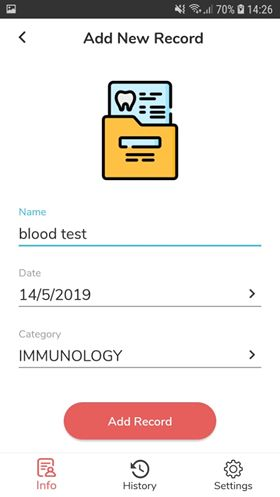
\includegraphics[width=7cm, height=13cm]{addNewRecord.jpg}
        \caption{Ecranul unde sunt completate datele}
        \end{figure}

    
    \item O cerere HTTP POST este apoi făcută către server.
    
    \begin{figure}[H]
        \centering
        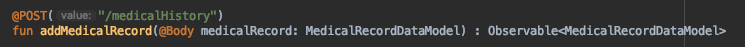
\includegraphics[width=15cm]{addMethod.png}
        \caption{Metodă HTTP și ruta la care se face cererea}
        \end{figure}

        \begin{figure}[H]
            \centering
            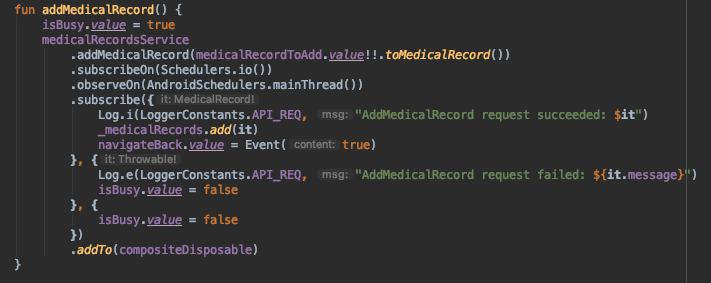
\includegraphics[width=15cm, height=7cm]{addRequest.png}
            \caption{Codul prin care se face cererea la server}
            \end{figure}


    \item În final datele ajung la server și sunt salvate în baza de date.
    

    \begin{figure}[H]
        \centering
        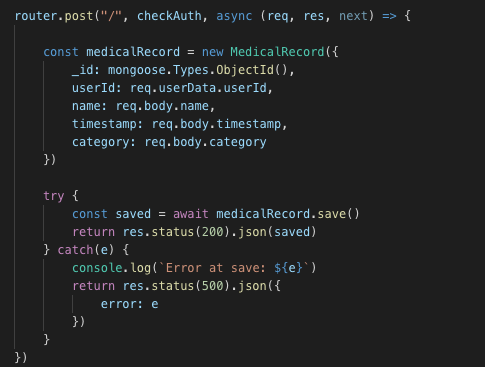
\includegraphics[width=10cm, height=6cm]{addServer.png}
        \caption{Cod din server}
        \end{figure}

\end{enumerate}

Datele care sunt salvate în memoria telefonului sunt datele generale ale utilizatorului care pot fi folosite
și fără conexiune la internet pentru modul de urgență. Ele sunt păstrate într-o baza de date locală criptată.
Sunt folosite și fișierele de preferință pentru a salva date de dimensiuni mici 
cu scop auxiliar. La fel că baza de date locală, și fișierele de preferințe sunt criptate.

\bigskip

\begin{figure}[H]
    \centering
    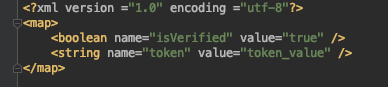
\includegraphics{noncript.png}
    \caption{Fișier de preferințe fără criptare}
    \end{figure}

    \begin{figure}[H]
        \centering
        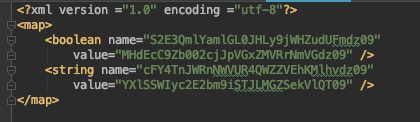
\includegraphics{cript2.png}
        \caption{Fișier de preferințe cu criptate}
        \end{figure}

\newpage
\subsection{Testarea}

Pentru a asigura calitatea soluției soft am dezvoltat în paralel cu aplicația 
și o suită de teste. Majoritatea testelor sunt de tip unitar, verificând o anumită
funtionalitate. De asemenea testele sunt separate în funcție de entitatea pe care o testează 
(serverul sau clientul).


Pentru a testa serverul REST făcut în Node.js am folosit o serie de pachete ajutătoare: 
mocha, chai și supertest. Am creat teste pentru rutele disponibile. Testele rulează într-o
configurarea separată care validează token-ul de autentificare în mod implicit.

\begin{figure}[H]
    \centering
    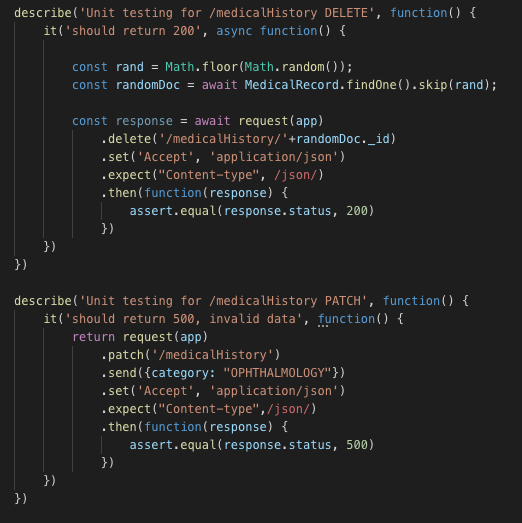
\includegraphics[width=10cm, height=8cm]{unitnode.png}
    \caption{Exemple de teste unitare în Node.js}
    \end{figure}


Pentru a rula un test pe o anumită ruta se definește ruta la care se va execută testul,
metodă (GET, POST, DELETE, etc\dots) și eventualele date de care e nevoie. Apoi se definește
ce cod ar trebuii să aibe răspunsul primit și eventual ce date sau tip de date ar trebuii primite.

\begin{figure}[H]
    \centering
    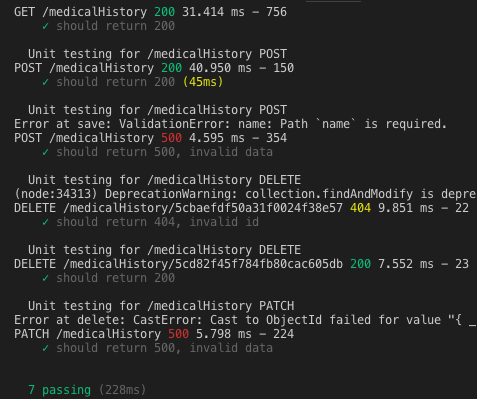
\includegraphics[width=8cm, height=6cm]{confnode.png}
    \caption{Rularea unei suite de teste pe ruta /medicalHistory}
    \end{figure}


Pentru clientul mobil am folosit JUnit, o librărie specilizate pe unit testing și
diferite librării auxiliare oferite de Kotlin și Android pentru a elabora și teste de integrare.

\begin{figure}[H]
    \centering
    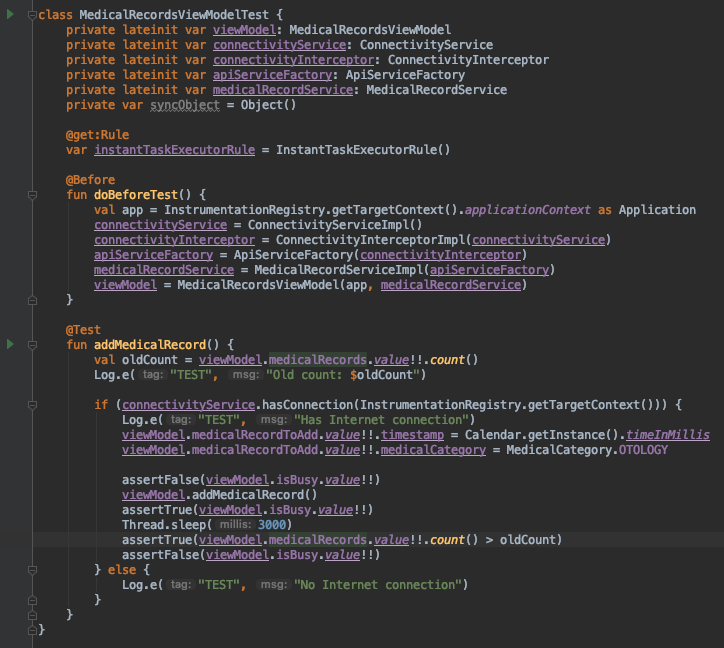
\includegraphics[width=10cm, height=8cm]{interg.png}
    \caption{Clasa cu test de integrare care cuprinde mai multe servicii și un ViewModel}
    \end{figure}


\newpage
\section{Concluzii}

Acestă lucrare a avut ca scop exemplificarea în mod practic și teoretic a anumitor probleme
pe care o aplicație mobilă le poate avea atunci când lucrează cu date personale.
Având în vedere mișcările din lumea politică și adopotarea unor legi precum GDPR, 
astfel de subiecte devin din ce în ce mai relevante pentru utilizatori dar și pentru
dezvoltatorii de aplicații. 

\bigskip

Aplicația Medicarium a fost dezvoltată că și un reper. Pas cu pas, de la proiectarea
aplicației până la testare, există decizii importante pe care trebuie luate pentru a asigura
integritatea, confidențialitatea și disponibilitatea datelor utilizatorilor.

\bigskip
Aplicația poate fi extinsă și imbunatatia, ce am tratat în lucrare nu cuprinde
amplul spectru a cea ce înseamnă securitate și confidențialitate. În lucrare am
observat câteva din cele mai importante etape a unei aplicații. O îmbunătățire
ar putea fi creare unui sistem de backup al datelor mai riguros. La momentul de față
singurul backup disponibil este la nivelul bazei de date. O altă îmbunătățire
ar putea fi extinderea modului offline astfel în cât să cuprindă toate funcționalitățile
aplicației, nu doar modul de urgență.

\bigskip

În concluzie, se recomandă ca dezvoltatorii de aplicații mobile să ia în serios
problematica securității și confidentialitații datelor, în caz contrar, se pot
lua măsuri legale care pot afecta în mod negativ compania sau persoană respectivă.

\newpage
\section{Bibliografie}
\nocite{owasp-top10-2017}
\nocite{owasp-top10-mobile}
\nocite{3ways-auth}

\nocite{liu2016follow}
\nocite{ssidloc}
\nocite{googleperm}
\nocite{redditcalc}

\nocite{rfc-7519}
\nocite{jwt}
\nocite{enisa-2017}
\nocite{enisa-security-data-processing}
\nocite{goldberg1998comparison}
\nocite{felt2017measuring}
\nocite{fette2011websocket}
\nocite{erkkila2012websocket}
\nocite{test-ws}

\nocite{katz1996handbook}
\nocite{tutrsa}
\nocite{jonsson2003public}

\nocite{kahn2010mobile}
\nocite{barton2012regulation}

\nocite{mvvmpng}

\nocite{masse2011rest}
\nocite{tilkov2010node}
\nocite{reqpersec}

\nocite{banker2011mongodb}
\nocite{nayak2013type}


\nocite{jetpackpng}
\nocite{statcounter}
\nocite{moskala2017android}
\nocite{kotlinvsjava}

\printbibliography[title=Bibliografie]

\end{document}